% !TeX spellcheck = en_UK
\documentclass[12pt,english]{report}
\usepackage{tesi}

\usepackage[a4paper]{geometry}		% Formato del foglio
\usepackage[english]{babel}
\usepackage[utf8]{inputenc}			% Supporto per UTF-8
\usepackage[a-1b]{pdfx}				% File conforme allo standard PDF-A (obbligatorio per la consegna)

\usepackage{graphicx}				% Funzioni avanzate per le immagini
\usepackage{hologo}					% Bibtex logo with \hologo{BibTeX}
\usepackage{epsfig}				    % Permette immagini in EPS
\usepackage{xcolor}                 % Gestione avanzata dei colori
\usepackage{amssymb,amsmath,amsthm} % Simboli matematici
\usepackage{listings}				% Scrittura di codice
\usepackage{url}					% Visualizza e rendere interattii gli URL
\usepackage[pdfa]{hyperref}			% Rende interattivi i collegamenti interni
\usepackage{tikz}                   % Permette di disegnare inline
\usepackage{import}
\usepackage{float}
\usepackage{xstring}                % Permette di usare la funzione \IfInteger
\usepackage{array}                  % Permette di usare colonne "m" dentro table
\usepackage{multirow}               % Permette di creare tabelle con righe multiple
\usepackage{caption}                % Roba per le figure side-by-side
\usepackage{subcaption}             % Roba per le figure side-by-side
\usepackage{enumitem}               % Gestione delle liste
\graphicspath{{imgs/}}
\usepackage{minted}
\usepackage{booktabs}

\usepackage[backend=biber, style=numeric]{biblatex}
\addbibresource{bibliography.bib}

\usetikzlibrary{positioning}
\usetikzlibrary{calc}
\usetikzlibrary{shapes}

\usepackage[autostyle = false]{csquotes}
\MakeOuterQuote{"}
\usepackage{setspace}
\usepackage{algorithm}
\usepackage[noEnd=true]{algpseudocodex}
\usepackage{etoolbox} 
\AtBeginEnvironment{algorithmic}{\setstretch{1.3}}

\newcommand{\GeneraSchemaPacchetto}[2]{{
		\begin{tikzpicture}
			[
			box/.style={draw,rectangle,minimum width=\recminwidth, 
				minimum height=\rectangleheight, 
				outer sep=0pt, node distance=0pt}
			]
			
			\def\rectangleheight{1cm}
			\def\recminwidth{2cm}
			
			\foreach \name/\size in {#1} {
				\node[box, label={below:\small \texttt{\size{} byte}}] (0) {\texttt{\name}};
			}    
			
			\foreach \name/\size [count=\i] in {#2}
			{
				\pgfmathtruncatemacro\prevposition{\i - 1}
				\node[box, right = 0pt of \prevposition,
				label={below:\small \texttt{\IfInteger{\size}{\size\ byte}{\size}}}
				] (\i) {\texttt{\name}};
			}
		\end{tikzpicture}
}}

\def\myCDL{Master's Degree Course in \\ Computer Science}

% TITOLO TESI:
%\def\myTitle{Smthng about Fuzzing, probably}
%\def\myTitle{Improving Coverage-Guided Fuzzing through Bloom Filter-Based Coverage Maps}
\def\myTitle{Evaluation of Bloom Filter-Based coverage Maps in Coverage-Guided Fuzzing}

% AUTORE:
\def\myName{Massimo Perego}
\def\myMat{ID Number 54204A}

% RELATORE E CORRELATORE: 
\def\myRefereeA{Prof. Andrea Lanzi}
\def\myRefereeB{Prof. Flavio Toffalini}

% ANNO ACCADEMICO
\def\myYY{2025-2026}

% Il seguente comando introduce un elenco delle figure dopo l'indice (facoltativo)
%\figurespagetrue

% Il seguente comando introduce un elenco delle tabelle dopo l'indice (facoltativo)
%\tablespagetrue

\theoremstyle{definition}
% \newtheorem{defin}{Definition}[section]
\newtheorem{defin}{Definition}


\begin{document}
	
	\frontespizio
	\afterpreface

    \chapter{Introduction}
\label{chap:intro}

As modern software systems become increasingly complex, their attack surface expands correspondingly, elevating software vulnerabilities to a critical security concern. The consequences of unpatched software flaws can range from isolated service disruption to systemic data breaches with global impact. Automated vulnerability discovery has therefore transitioned from an academic pursuit to a fundamental necessity within the software development life cycle. While techniques such as static analysis \cite{nachtigall2022large} and symbolic execution \cite{baldoni2018survey, king1976symbolic} provide valuable insights and high precision, practical constraints regarding scalability and path explosion can make them less effective in large systems. In contrast, dynamic analysis --- and more specifically, fuzz testing or "fuzzing" --- has emerged as the remarkably pragmatic and dominant approach for identifying flaws in compiled binaries.

Coverage-Guided Fuzzing (CGF) has established itself as the \textit{de facto} standard for automated software testing. Evolving from early blind random-input generators \cite{miller1990empirical} to highly sophisticated feedback-driven engines \cite{fioraldi2020afl++, honggfuzz, libfuzzer}, fuzzing is now deployed on an industrial scale. It is responsible for discovering thousands of critical vulnerabilities across diverse domains, including general open-source applications \cite{ossfuzz}, Internet of Things (IoT) devices \cite{chen2018iotfuzzer, zheng2019firm}, operating system kernels \cite{syzkaller, xu2020krace}, and enterprise-level database systems \cite{jiang2023dynsql, liang2024wingfuzz, wang2021reinforcement}. Modern fuzzers rely on the continuous aggregation of execution telemetry to guide the generation of new test cases. By monitoring the control-flow graph (CFG) transitions triggered by mutated inputs, the fuzzer can actively prioritise inputs that discover previously unseen code paths, effectively exploring the target application's state space.

Despite its undeniable success, the efficacy of any CGF engine is fundamentally bound by the quality and granularity of the feedback guiding it \cite{wang2019sensitive}. The fuzzer relies on coverage metrics as a proxy for program state exploration. For this reason, several new techniques have been developed recently to overcome the limitations of CGF, such as hard-to-bypass constraints \cite{aschermann2019redqueen, poeplau2020symbolic, stephens2016driller, yun2018qsym} and the high number of invalid test cases generated by mutation \cite{aschermann2019nautilus, blazytko2019grimoire, fioraldi2020weizz, padhye2019semantic}. These modifications are all designed to maximise code coverage, as exploring a greater proportion of the codebase is empirically proven to yield a higher rate of flaw discovery.

Modern fuzzers predominantly rely on edge coverage \cite{manes2019art} rather than simple basic block coverage. By tracking the specific control-flow transitions between blocks, edge coverage provides the fuzzer with more granular feedback on the program's internal state. This is traditionally implemented by assigning a unique identifier to each branch transition \cite{zalewski2014afltech}, allowing the engine to quickly record and recognise newly discovered execution paths during the fuzzing loop.

Indirect branches pose a uniquely complex challenge within this tracking mechanism. Unlike direct branches, where the target address is statically known, an indirect branch --- such as a function pointer invocation, a virtual method dispatch in C++, or a complex switch-case statement --- dynamically resolves its destination at runtime based on register states or memory contents. Consequently, a single indirect call site can map to numerous diverse targets, significantly increasing the number of edge transitions that must be tracked.

To overcome this limitation, this thesis proposes and evaluates a new architectural enhancement for AFL++: the introduction of a secondary coverage map dedicated exclusively to tracking the targets of indirect control-flow transfers. We hypothesise that indirect branch tracking might provide the fuzzer with a higher-fidelity representation of the program's dynamic execution state, thereby improving overall path discovery.

The core tenets of the proposed architecture are:
\begin{itemize}
    \item \textit{Isolation:} Indirect branch data is stored in an independent shared memory region, preventing interference with the primary edge coverage bitmap and preserving standard edge discovery.

    \item \textit{Collision-Free Identification:} The architecture employed guarantees that every indirect branch source in the binary is mapped to a unique slot.

    \item \textit{Probabilistic Tracking:} To maintain strict memory and performance bounds, each indirect source slot acts as a Bloom filter containing already-seen transitions. 

    \item \textit{Dynamic Sizing:} The required capacity of the secondary map is computed iteratively at startup by the instrumented binary and communicated to the fuzzer, ensuring optimal memory utilisation.
\end{itemize}

We implemented this architecture by extending the LLVM compiler infrastructure to inject tracking logic at the site of every indirect jump and call, modifying the compiler-rt libraries to handle runtime initialisation, and altering the fuzzer's core orchestration to accommodate dynamic memory reallocation and dual-map seed scoring.

Following the implementation, an empirical evaluation was conducted using a diverse set of real-world benchmarks to assess the impact of the indirect coverage map on path discovery and fuzzing throughput. The results of this evaluation indicate that, while the proposed architecture functions mechanically as intended, it did not yield the anticipated breakthrough in overall coverage growth. Across all tested benchmarks, the baseline AFL++ consistently performed either on par with or slightly better than the modified architecture.

This thesis explicitly details these negative results and provides insight into the possible structural and theoretical limitations that caused them. We establish that the lack of improvement is primarily attributable to redundancy with the primary edge map. Furthermore, we identify limitations within the standard mutation engine, which struggles to generate the precise data structures (e.g., valid pointers) necessary to satisfy complex indirect dispatch constraints without the aid of specialised techniques \cite{aschermann2019redqueen}. Additional advanced taint-tracking approaches \cite{wang2010taintscope} might be required to fully leverage indirect paths.

\section{Contributions}

The primary contributions of this thesis are:
\begin{itemize}
    \item A comprehensive analysis of the limitations of traditional, fixed-size shared memory bitmaps in tracking indirect control-flow within Coverage-Guided Fuzzing.

    \item The design and implementation of an isolated, dynamically sized secondary coverage map for AFL++, providing collision-free tracking of indirect branch sources.

    \item An empirical evaluation of the proposed architecture against standard baselines, accompanied by a critical analysis of the structural limitations.
\end{itemize}

\section{Thesis Structure}

In Chapter \ref{ch:bg}, we provide the necessary background on automated software testing, detailing the terminology and a general description of fuzz testing. In Chapter \ref{ch:afl}, we dissect the architecture of AFL++. In Chapter \ref{ch:arch}, we present the theoretical design of the proposed architecture. In Chapter \ref{ch:impl}, we detail the concrete engineering modifications made to the AFL++ codebase. In Chapter \ref{ch:eval}, we present the results and analyse the observed outcomes. The thesis ends with Chapter \ref{ch:concl}, containing conclusions and the discussion for possible future directions.

    \chapter{Foundations of Vulnerability Discovery}
\label{ch:bg}

The fundamental challenge of software security is the identification of unintended, exploitable states. Given the complexity of non-trivial codebases, exhaustive manual auditing is infeasible.

To automate vulnerability discovery, three primary approaches have emerged: static analysis, symbolic execution, and dynamic analysis, most notably, fuzzing. While each methodology offers unique advantages, practical constraints regarding scalability and precision have established fuzzing as the dominant approach for identifying flaws in compiled binaries.

\subsubsection{Static Analysis}

Static Application Security Testing (SAST) relies on examining source code, bytecode, or binaries, to identify issues via a pre-defined set of syntactic or semantic rules without ever executing the program. This enables the identification of security concerns early in the development cycle --- long before the code is deployed --- and theoretically allows for the evaluation of all possible execution paths by traversing the program's abstract syntax tree (AST) or control flow graph (CFG).

However, the pursuit of comprehensiveness in static analysis requires conservative assumptions about the runtime state. This can become particularly problematic when attempting to resolve dynamic memory allocations, pointer aliasing, and dynamic control flow. 

The necessary over-approximation of the program's behaviour leads to a high volume of false positives \cite{nachtigall2022large}. Furthermore, the reliance on pre-defined rule sets can miss bugs that deviate, even slightly, from known vulnerability patterns.

\subsubsection{Symbolic Execution}
 
Symbolic execution addresses the precision failures of static analysis by exploring paths using symbolic variables rather than concrete values \cite{king1976symbolic}. The engine builds a logical formula representing the constraints required to reach specific execution paths. An SMT (Satisfiability Modulo Theories) solver is then used to determine whether a path is reachable. 

% sound = can check that there are no errors, zero false negatives/never misses real bug, might be false positives
% complete = if it reports a bug it's real, zero false positives, might be false negatives

While providing rigorous formal guarantees for the paths it does explore, symbolic execution suffers from severe scalability issues: 
\begin{itemize}
    \item Path Explosion: The number of paths in a program grows exponentially with the number of conditional branches (and infinitely in the presence of unbounded loops), frequently causing the state space to grow beyond computational feasibility.

   \item Constraint Solving Complexity: SMT solvers struggle with non-linear arithmetic and complex memory models. When encountering these constructs, the solver can slow down significantly or even time out, halting exploration.
\end{itemize}
Due to these problems \cite{baldoni2018survey}, symbolic execution is generally considered incomplete (since not all paths can be explored) but highly precise.

\subsubsection{The Pragmatism of Coverage-Guided Fuzzing}

Coverage-Guided Fuzzing (CGF) operates entirely in the realm of concrete execution. By feeding mutated, real inputs to a target and monitoring the execution, fuzzers sidestep the need for mathematical abstractions and constraint solving.

The primary advantages of this method are:
\begin{itemize}
    \item Concrete Reproducibility: Each reported crash or violation is guaranteed to be real, as it is accompanied by a concrete test case that triggers the fault.

    \item Scalability: Fuzzing is inherently highly parallelizable and often bound only by the target's execution speed.
\end{itemize}
However, since it relies primarily on random mutation to navigate the program's state space, the coverage feedback mechanism is essential to prevent the technique from devolving into a blind search.

\section{Terminology}

\begin{defin}[Fuzzing]
    \textit{Fuzz testing} or \textit{Fuzzing} is the action of running a program using inputs sampled from an input space that may exceed the expected input space, to trigger unintended behaviour \cite{manes2019art}.
\end{defin}

\begin{defin}[Fuzzer]
    A \textit{Fuzzer} is a program that performs fuzz testing on a target.
\end{defin}

\begin{defin}[Coverage-Guided Fuzzing]
    \textit{Coverage-Guided Fuzzing} (CGF) is a feedback-driven fuzzing approach that uses control flow transitions to evaluate the impact of each mutated input \cite{zalewski2014afltech}.
\end{defin}

\begin{defin}[Control Flow Graph]
    A \textit{Control Flow Graph} (CFG) is an abstraction of the control flow behaviour of a program. The CFG is a directed graph where the vertices represent basic blocks and edges represent possible control flow transfers \cite{allen1970control}.
\end{defin}

\begin{defin}[Basic Block]
    A \textit{Basic Block} is a sequence of code with only one entry point and a single exit point \cite{gccinternals}.
\end{defin}

\begin{defin}[Edge]
    Each \textit{Edge} is a link between basic blocks, representing a possible control flow transfer from the end of a basic block to the head of another \cite{gccinternals}.
\end{defin}

\begin{defin}[Direct Jump]
    A \textit{Direct Jump} is a control flow transition in which the target is statically defined.
\end{defin}

\begin{defin}[Indirect Jump]
    An \textit{Indirect Jump} is a control flow transition in which the target is only determined at runtime.
\end{defin}

\begin{defin}[Instrumentation]
    \textit{Instrumentation} is defined as the process of augmenting a target program with modifications. This typically involves the insertion of lightweight logic to extract execution feedback, such as edge coverage, without altering the program's intended semantics.
\end{defin}

\begin{defin}[Coverage Map]
    The \textit{Coverage Map} is a data structure typically implemented as a shared memory region between the fuzzer and the instrumented binary \cite{zalewski2014afltech}. It records basic block transitions and is used by the fuzzer to track the execution paths triggered by a specific input.   
\end{defin}

\begin{defin}[Map Collision]
    A \textit{Map Collision} is an overlap in the coverage map, occurring when two distinct control flow edges are mapped to the same index in the coverage map. 
\end{defin}

\begin{defin}[Seed]
    A \textit{Seed} is a concrete input file or byte sequence provided to a fuzzer and executed against the target program.
\end{defin}

%\begin{defin}[Seed Corpus]
%   The \textit{Corpus} is a maintained collection of known inputs that the fuzzer uses as a baseline for mutation. This is dynamically updated as new coverage-yielding seeds are discovered.
%\end{defin}

\section{Fuzzing Fundamentals}
\label{sec:ff}

Since it was first proposed in 1990 \cite{miller1990empirical}, fuzzing has established itself as a standard method for automated vulnerability detection. At its core, fuzzing involves the iterative generation of malformed test cases to explore the input space of an application with the aim of triggering unintended program behaviour. 

The assumption is that if an application's input validation cannot gracefully handle unexpected inputs, those inputs may expose vulnerabilities. Various fuzzing techniques have been proposed \cite{aschermann2019nautilus, chen2018angora, dutra2023formatfuzzer}, developed \cite{honggfuzz, libfuzzer, zalewski2014afltech}, and used effectively to identify a large number of vulnerabilities \cite{honggfuzzbugs, syzkallerbugs, rashbugs}.

\subsection{Components of a Fuzzer}

While fuzzing techniques can vary widely in their implementation, most modern fuzzers share a common set of basic entities \cite{fioraldi2022libafl}.

\paragraph{Input} The fuzzer's internal representation of data, which may differ from the format the program actually consumes. Simple fuzzers manipulate input as raw bytes, while more advanced engines work with more complex structures --- such as Abstract Syntax Trees \cite{aschermann2019nautilus} or system calls \cite{syzkaller} --- to modify the data while maintaining its validity. 

\paragraph{Corpus} A fuzzer's corpus stores inputs and their metadata, typically either in memory or on disk. Fuzzing models generally require at least two corpora: one used to evolve interesting test cases, and another for saving successful solutions (i.e., crashes).

\paragraph{Scheduler} Strictly tied to the corpus, it determines which test cases should be evaluated next. Basic implementations might rely on a FIFO queue or random selection, while more complex schedulers use heuristics to prioritise more valuable inputs \cite{chen2020meuzz, rebert2014optimizing, wang2021reinforcement}.

\paragraph{Stage} A component that executes one or more specific actions --- such as mutation, analysis, or minimisation --- on a single test case.

\paragraph{Observer} An observer provides data from an execution of the target program, which is used to efficiently analyse the execution itself. A common example of an observer is the coverage map, although other types exist \cite{aschermann2020ijon, padhye2019fuzzfactory}.

\paragraph{Executor} The component responsible for actually executing the target, which defines all operations related to a single run of the target program with the given input. It can vary in complexity, from a call to a harness \cite{libfuzzer} to restarting an operating system from a snapshot \cite{schumilo2021nyx}.

\paragraph{Feedback} Feedback is used to classify the outcome of an execution as interesting or not. It processes the information given by one or more observers. 

\paragraph{Mutator} The mutator is responsible for generating new inputs through the transformation of one or more existing inputs. These operators can be random or format-aware, enabling them to manipulate the input's internal representation \cite{wang2019superion}.

\paragraph{Generator} A component designed to generate new inputs from scratch. It can be completely random or grammar-based \cite{aschermann2019nautilus}.

\begin{figure}
    \centering
    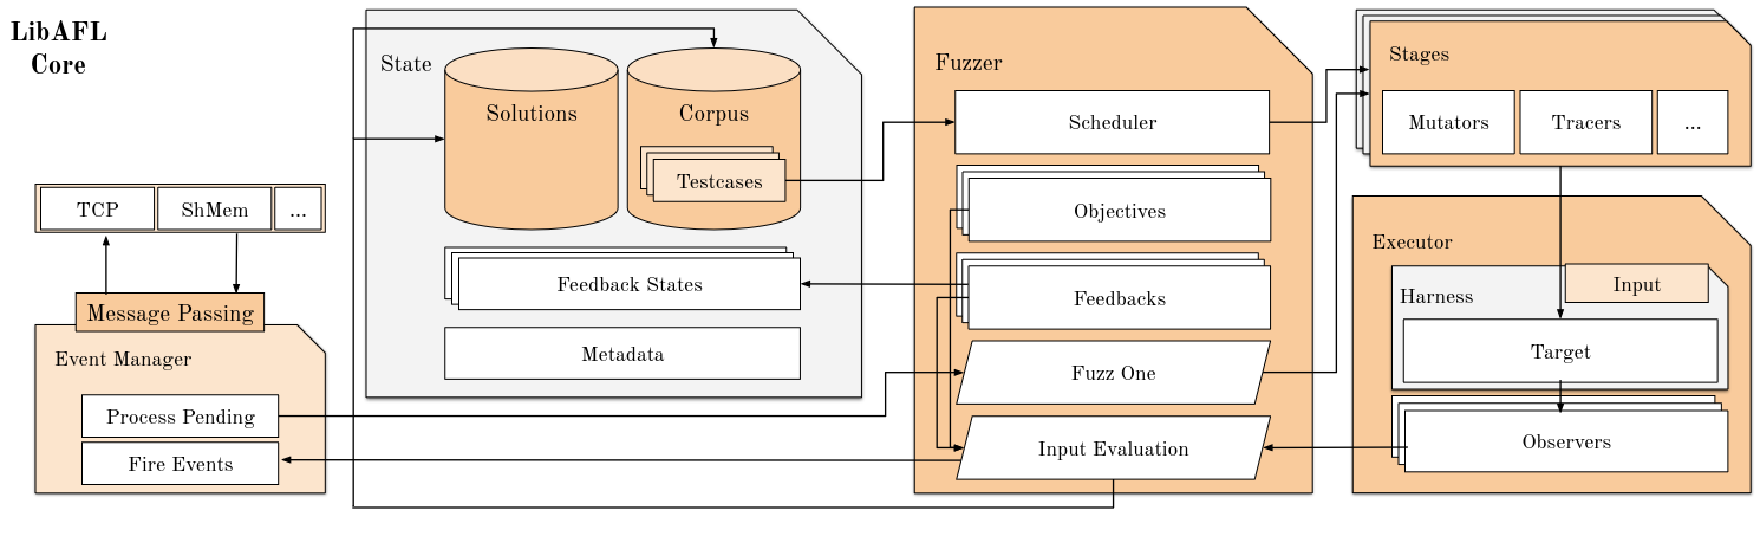
\includegraphics[width=\linewidth]{imgs/background/libaflcore.pdf}
    \caption{\textsc{LibAfl} core architecture, as shown in \cite{fioraldi2022libafl}, Figure 1}
    \label{fig:libaflcore}
\end{figure}

\subsubsection{Core Fuzzing Loop}

All feedback-driven fuzzers share a common core loop, which can be decomposed into four main stages:
\begin{enumerate}
    \item \textbf{Input generation and scheduling}: The scheduler chooses an input from the corpus to be passed on to the mutator.

    \item \textbf{Execution}: The new candidate input is injected into the target program, in a manner defined by the executor.

    \item \textbf{Feedback evaluation}: The information collected during execution is used to determine whether an input is interesting. The definition of ``interesting'' is abstract, but is always correlated with novelty in the search (e.g., new code or edge coverage).

    \item \textbf{Corpus update}: The set of interesting test cases and solutions is updated according to the feedback. The cycle then repeats.
\end{enumerate}

\subsection{Fuzzer Classification}

The taxonomy of fuzzers is traditionally established along two main criteria: the methodology for test case generation and the level of visibility into the target program.

\paragraph{Based on Input Generation} The first classification criterion relies on how test cases are produced, generally dividing fuzzers into two categories:
\begin{itemize}
    \item \textbf{Generation-based} fuzzers create new test cases from scratch, using a specification of the input format, e.g., a model \cite{peachfuzzer} or block \cite{aitel2002advantages}.

    \item \textbf{Mutation-based} fuzzers rely on a pre-existing corpus, which must be provided in the initial state.
\end{itemize}

\paragraph{Based on Target Knowledge} This criterion evaluates the extent to which a fuzzer can observe the internal state and execution paths of the target program. This traditionally divides fuzzers into three categories \cite{liang2018fuzzing}:
\begin{itemize}
    \item \textbf{Black-box} fuzzers treat the target application as an opaque system, interacting with it solely through input/output channels and observing external outcomes, such as crashes or hangs. These are closely related to random testing. However, a lack of information about the target's implementation does not imply a lack of specification knowledge; black-box fuzzers might still require a model of the input format to generate test cases.

    \item \textbf{White-box} fuzzers possess complete visibility of the target's internals, typically employing techniques such as symbolic execution to leverage constraints found during execution \cite{godefroid2008automated}.

    \item \textbf{Grey-box} fuzzers represent a middle ground, collecting minimal information to better explore the input space while limiting performance overhead. This feedback is typically based on code coverage and is collected through instrumentation \cite{zalewski2014afltech}.
\end{itemize}

\subsection{Coverage-Guided Fuzzing}

Empirical data \cite{ossfuzz} strongly suggests that integrating code coverage feedback into the fuzzing process increases overall efficiency, thereby yielding a higher number of faults discovered in a fixed time window.

There are many fuzzers that rely on code coverage as feedback, but the technique is not limited to this type of information \cite{aschermann2020ijon, wang2019sensitive}.

Fuzzers typically employ evolutionary algorithms to analyse execution feedback obtained from the target program, using this data to guide subsequent input generation. A general version of these algorithms is presented in Algorithm \ref{alg:evolfuzzing}.

\begin{algorithm}
\caption{Basic Evolutionary Fuzzing}\label{alg:evolfuzzing}
    \begin{algorithmic}[1]
    \State $F \gets \emptyset$ \Comment{Set of faults found}

    \State $S[C] \gets InitialCorpus$ \Comment{$S$ represents the fuzzer state}

    \While{\Call{ContinueFuzzing}{$S$}}
        \State $t \gets \Call{SelectTestcase}{S[C]}$ 
    
        \State $N \gets \Call{Calibrate}{t, S}$ \Comment{Determines time spent on $t$}
    
        \For{$i \gets 1$ \textbf{to} $N$}
            \State $t' \gets \Call{Mutate}{t}$ 
        
            \State $Tr \gets \Call{Execute}{T, t'}$ \Comment{Run target and obtain execution trace}

            \If{\Call{IsViolation}{$Tr, t'$}}
                \State $F \gets F \cup \{t'\}$
            \EndIf

            \If{\Call{IsInteresting}{$Tr, S$}}
                \State $S[C] \gets S[C] \cup \{t'\}$
            \EndIf
        \EndFor
    \EndWhile
    \Return{$F$}
\end{algorithmic}
\end{algorithm}

Code coverage is an abstract concept that, in the literature, is typically evaluated using one of three elements: basic blocks, basic block paths and, most commonly, basic block edges \cite{fioraldi2020afl++, honggfuzz, libfuzzer, zalewski2014afltech}. Tracking edges is the most common approach as it allows more granular tracking than simple block coverage, distinguishing between different traces spanning the same basic blocks, while avoiding problems such as path explosion.

For source-available binaries, code coverage is generally measured through instrumentation at compile time \cite{honggfuzz, zalewski2014afltech}. For source-unavailable binaries, feedback can be obtained via instrumentation inserted dynamically \cite{fioraldi2020afl++, rawat2017vuzzer}, or statically through binary rewriting \cite{dinesh2020retrowrite}.

    \chapter{Anatomy of a Modern Fuzzer}
\label{ch:afl}

While the components outlined in Section~\ref{sec:ff} establish the blueprint for most feedback-driven fuzzers, translating this architecture into a performant tool capable of operating at an industrial scale requires highly specific engineering implementations. The cycle of scheduling inputs, executing the target and evaluating feedback demands heavy performance optimisations to maintain efficiency in real-world usage.

AFL++ \cite{fioraldi2020afl++} has established itself as the \textit{de facto} standard in modern coverage-guided grey-box fuzzing. By consolidating diverse research advancements (such as \cite{aschermann2020ijon}, \cite{aschermann2019redqueen} and \cite{bohme2016coverage}) into a single project, it serves as the premier baseline for contemporary vulnerability research. Understanding the architectural choices provides context that is fundamental to identifying constraints that limit traditional edge coverage metrics.

\section{Compilation and Instrumentation}
\label{sec:compandinst}

Without execution telemetry, a fuzzer is essentially blind. To achieve visibility, the fuzzer must inject monitoring logic into the target program. Implementing an observer generally involves modifying the binary to report every basic block transition traversed during the execution via instrumentation.

However, instrumentation is not a monolithic process. In AFL++, there are multiple compile-time strategies available, which heavily dictate both the accuracy of the resulting coverage map and the performance overhead of the fuzzing loop.

AFL++ introduces three distinct compilation modes:
\begin{itemize}
    \item \textit{LLVM Mode}: Operates at the LLVM IR level, removing the need for assembly rewriting. It provides efficient basic-block instrumentation while laying the groundwork for more advanced features.
    
    \item \textit{LTO Mode}: Uses Link-Time Optimization to guarantee a collision-free coverage bitmap.

    \item \textit{GCC Plugin Mode}: It uses GCC compiler plugins, since not all codebases can be easily migrated to the LLVM infrastructure. It provides an essential, high-performance bridge without requiring a compiler toolchain overhaul.
\end{itemize}

In scenarios where source code is unavailable (such as proprietary or legacy software) AFL++ leverages emulation or dynamic binary instrumentation --- such as QEMU or FRIDA --- to inject execution tracking logic at runtime, accepting higher performance overhead for maintaining visibility.

\subsection{LLVM Mode}
\label{sub:llvmmode}

LLVM mode --- typically invoked using the flag \texttt{--afl-llvm}, the environment variable \texttt{AFL\_CC\_COMPILER=LLVM}, or via the compiler wrappers \texttt{afl-clang-fast} and \texttt{afl-clang-fast++} --- serves as the modern standard for instrumenting source-available targets.

This mode operates strictly at the LLVM Intermediate Representation (IR) level, removing the need for brittle assembly rewriting. Consequently, this allows the compiler to treat injected instrumentation as native code, allowing standard optimisation passes to optimise it alongside the target program and reduce performance overhead. Furthermore, operating at the IR level also means that the instrumentation is architecture-agnostic and generally independent of the target CPU architecture.

To fully leverage the LLVM framework, AFL++ implements its instrumentation as a custom LLVM compiler pass. Passes execute all transformations and optimisations of the compiler, compute the analysis results required by these operations, and serve as the architectural framework for compiler code \cite{writingllvmpass}.

The compiler wrappers work as drop-in replacements for the standard C/C++ compilers. When invoked, they execute the standard Clang compiler but instruct it to load AFL++'s custom shared object --- the instrumentation pass --- during the intermediate compilation pipeline. The final linking phase is equally important, as the compiler wrapper links the static library for the compiler runtime, whose primary responsibility is setting up the shared memory region for the coverage map and initializing the forkserver. 

\subsubsection{PCGUARD Instrumentation}

AFL++ heavily leverages and extends LLVM's \texttt{SanitizerCoverage} infrastructure. Rather than manually traversing the CFG to find every edge, AFL++'s \texttt{SanitizerCoveragePCGUARD.so.cc} pass performs the following:
\begin{enumerate}
    \item \textit{Block selection and pruning:} The pass iterates over all basic block structures in a function, then uses Dominator and Post-Dominator trees to identify blocks where coverage tracking is redundant (e.g., a block that has a single predecessor and a single successor). These blocks can be skipped \cite{agrawal1994dominators} to reduce overhead.

    \item \textit{Guard Allocation:} For every instrumented block, the compiler reserves a 32 bit slot in a dedicated ELF section (\texttt{\_\_sancov\_guards}). At compile-time, these are uninitialized integers. 

    \item \textit{Inline IR Injection:} For each selected basic block, LLVM IR is injected at the start of the block:
    \begin{itemize}
        \item It creates an \texttt{IntToPtr} lookup into the \texttt{sancov\_guards} array using a unique index for that block.
        
        \item It loads the 32-bit coverage ID from that guard slot.
        
        \item It uses a \texttt{GetElementPtr} (GEP) instruction to calculate the exact byte address within the \texttt{\_\_afl\_area\_ptr} (the shared memory map bridging the fuzzer and target) using the loaded coverage ID.
        
        \item It loads the current 8-bit counter from that shared memory byte, increments it, and stores it back.
    \end{itemize}
    See Appendix \ref{app:llvmir} for an example of standard injected LLVM IR.
\end{enumerate}

\paragraph{Initialisation of Guards} The mode relies on an array of guard variables, which must be initialised at runtime. The compiler groups all \texttt{\_\_sancov\_guards} across different translation units. At load time, a constructor function provided by the compiler runtime is executed (\texttt{\_\_sanitizer\_cov\_trace\_pc\_guard\_init}). This runtime function iterates over all 32-bit guard pointers, assigning a random pseudo-unique ID to each one, bounded by the shared memory size. This allows mapping the CFG basic blocks to random slots in the fuzzer's shared bitmap.

\subsubsection{Classic Tracing}

When PCGUARD is not available, AFL++ falls back to "Classic" tracing mode. The pass \texttt{afl-llvm-pass.so.cc} computes edge coverage using the original AFL coverage formula \cite{zalewski2014afltech}:
\[
    \text{map}[\text{cur\_loc} \oplus (\text{prev\_loc} \gg 1)] \mathrel{{+}{=}} 1
\]

In this design, \texttt{cur\_loc} is a pseudo-random identifier statically assigned at compile-time, while \texttt{prev\_loc} holds the identifier of the previously executed block. To maintain execution context across the program, the injected instrumentation must save the current block's identifier into a thread-local variable before transferring control flow to the subsequent block.

The bitwise right shift ($\gg 1$) is necessary to distinguish edge $A \rightarrow B$ from $B \rightarrow A$, since the XOR operation is commutative. Not modifying one of the operands would result in symmetric transitions, losing the sequence's directionality. It also prevents self-loops ($A \rightarrow A$) from always being mapped to index 0.

\subsection{LTO Mode}

In standard LLVM mode, every C/C++ source file (translation unit) is compiled and instrumented entirely independently, with no view of the global program. This inevitably leads to map collisions when linking multiple object files, as random basic block IDs might overlap.

Link-Time Optimization (LTO) mode addresses this inefficiency by shifting the instrumentation process to the final linking phase. By operating with global visibility, the AFL++ LTO instrumentation pass (\texttt{SanitizerCoverageLTO.so.cc}) can uniquely identify each edge. As a result, LTO mode guarantees a collision-free coverage bitmap. By eliminating index overlaps, the fuzzer receives better edge coverage granularity, improving the accuracy of the feedback loop.

However, these benefits are tied to stricter toolchain requirements, requiring LLVM version 12+ to natively allow the LLVM linker to load plugins.

\paragraph{The LTO Solution} With this mode, AFL++ defers final compilation and optimization until the linking phase, intercepted via the compiler wrappers \texttt{afl-clang-lto} and \texttt{afl-clang-lto++}.

When compiling source code with the wrappers, the compiler passes the \texttt{-flto=full} flag to LLVM, instructing it to emit LLVM bitcode instead of the final machine code.

At link time, the custom linker \texttt{afl-ld-lto} invokes AFL++'s specialized linker pass. With global visibility into the CFG of the entire program, there is no need for random IDs, instead, it iterates through every block across the entire binary and assigns a contiguous, monotonically increasing identifier to every edge.

\subsubsection{LTO-Exclusive Features}

\paragraph{Autodictionary} By analysing the whole program at once, the linker can see every single constant string across all linked libraries and object files. During the LTO pass, it automatically scrapes these strings and generates a binary dictionary structure explicitly embedded within a specific ELF section of the target binary.

The AFL++ runtime extracts this dictionary when starting the target, immediately integrating it into its mutation strategies.

\paragraph{Fixed Memory Map Address} To eliminate the overhead associated with dynamically looking up the shared memory map pointer in the Global Offset Table (GOT), LTO mode can hardcode the absolute memory address of the shared memory region directly into the assembly of the coverage instructions. 

This can crash targets that utilize early constructors, deferred forkservers or anything that might conflict with OS memory layout or ASLR.

\paragraph{Document Edge IDs} The compiler outputs a comprehensive mapping of every assigned Edge ID to its corresponding function and file name.

\subsection{GCC Plugin Mode}

LLVM and LTO modes inherently rely on the target software being compatible with the LLVM compiler toolchain. In practice, not all codebases can be easily migrated to the LLVM infrastructure. Legacy systems and heavily architecture-dependent projects often cannot be compiled using Clang.

To maintain efficient execution insights, AFL++ incorporates the GCC plugin mode, replacing the assembly-level rewriting approach of the original \texttt{afl-gcc}. Instead of inserting assembly blocks directly into the compiled output, this mode operates at the compiler level via true GCC plugins. This ensures that the target can still benefit from compile-time instrumentation and optimisations while remaining tied to the GCC ecosystem.

To build with \texttt{afl-gcc-fast}, the host system must have GCC version 4.5.0 or newer and the corresponding \texttt{gcc-VERSION-plugin-dev} installed.

\paragraph{GIMPLE Pass Injection} The GCC compiler uses several intermediate representations, most notably GIMPLE \cite{gccinternals}. The AFL++ plugin registers a custom pass that operates on the GIMPLE trees. The pass \texttt{afl-gcc-pass.so.cc} acts as a GIMPLE pass which iterates over all basic blocks within a function and: 
\begin{enumerate}
    \item Assigns a random integer ID to all basic blocks.

    \item Constructs GIMPLE statements to calculate the standard AFL edge coverage formula.

    \item Emits a GIMPLE memory load/store sequence to increment the corresponding byte in the \texttt{\_\_afl\_area\_ptr} shared memory map.
\end{enumerate}

Because it relies strictly on GCC's plugin API and GIMPLE, this mode lacks the deeper analysis features found in LLVM, such as LAF-Intel (Split Compares), autodictionary and context-sensitive coverage.

\subsection{Black-Box Binary Instrumentation}
\label{subsec:bbb-instr}

When source-code is unavailable, compile-time instrumentation is impossible. To fuzz a black-box binary efficiently, dynamic binary instrumentation (DBI) or static binary rewriting is required. 

AFL++ offers extensive support for binary-only targets through several modes and integrations. The choice of mode depends largely on architecture, operating system, performance requirements and stability of the target. 

FRIDA or QEMU mode with persistent mode are the fastest, provided stability is high enough.

\subsubsection{QEMU Mode}

QEMU mode utilizes a patched version of QEMU running in user space emulation to instrument black-box, closed source binaries dynamically. It translates the target binary instructions into Tiny Code Generator (TCG) intermediate representation and injects AFL++ coverage collection instrumentation.

AFL++ can hook directly in the translation phase from machine code into TCG. When a new basic block is encountered and translated, the equivalent of the AFL coverage logging instruction is injected into the TCG block. Once translated, these cached blocks execute natively on the host.

\paragraph{Persistent Mode} It's the most significant performance enhancement, speeding up execution by several factors. This mode allows a target loop to be executed continuously within the same process, without forking for every attempt.

\subsubsection{FRIDA Mode}

This mode is an alternative to QEMU mode, usually with comparable performance, if not slightly faster. It is designed to be a drop-in replacement for QEMU mode, mimicking its environment variables (replacing \texttt{QEMU} with \texttt{FRIDA} in the name).

FRIDA mode operates by injecting a shared library \texttt{afl-frida-trace.so} into the target process. This relies on the \texttt{frida-gum} devkit and its dynamic translation engine ``\textit{Stalker}''.

Instead of full emulation, Stalker dynamically translates code basic block by basic block, injecting assembly snippets directly into the translated blocks. This model allows the fuzzer to inject execution tracking logic directly into the memory space of a running process.

\paragraph{FASAN: FRIDA Address Sanitizer Mode} Unlike QEMU mode --- which crashes if combined with ASAN --- FASAN allows injecting the same memory safety constraints at runtime. The dynamic loader intercepts standard memory functions and FRIDA dynamically instruments all memory operand instructions in the target binary, inserting calls provided by the ASAN dynamic shared object to validate read/writes operations against the shadow memory.

\subsubsection{Other Modes}

\paragraph{Nyx Mode} This mode shifts the paradigm to full-system emulation. Built upon a modified KVM and QEMU hypervisor, Nyx is designed to handle complex, stateful targets, kernel components or targets that cannot utilize persistent mode. Instead of utilizing forks, it utilizes KVM-based snapshots to revert the VM state.

\paragraph{Unicorn Mode} It's based on the Unicorn Engine, a fork of QEMU, and the instrumentation is, therefore, very similar. While QEMU provides a full Linux user-space environment, Unicorn Mode provides no environment at all; it simply emulates CPU instructions. Consequently, this mode requires writing a custom runtime harness to handle all memory mapping, register initialization, and syscall interception manually.

\paragraph{CoreSight Mode} This is AFL++'s hardware-assisted tracing solution, specifically designed for Arm64 architectures. It leverages ARM CoreSight technology to use the physical CPU's hardware trace macrocells to record control flow execution \cite{shan2023crowbar}. The CPU directly writes execution branch data into memory, which then has to be decoded. 

\paragraph{Binary Rewriters} These are external tools that can inject AFL++ coverage instrumentation directly into the binary either statically on disk --- such as ZAFL \cite{nagy2021breaking}, RetroWrite \cite{dinesh2020retrowrite} or Mcsema \cite{dinaburg2014mcsema} --- or dynamically at load/run time --- such as Dyninst \cite{buck2000api}.

\section{Runtime Components}

Compilation and instrumentation equip the target binary with the tools to report execution paths, but once visibility into the target is established, the challenge of CGF shifts to execution throughput. Processing millions of mutated inputs via standard system execution flows can introduce heavy performance bottlenecks.

The fuzzer requires an execution environment capable of managing the fuzzing loop, delivering mutated inputs, and evaluating the target's behaviour at scale. To achieve efficiency, modern fuzzers use high-speed inter-process communication (IPC) and specialized state management.

\subsection{The Forkserver Architecture}

The normal system execution flow for executing a program is to call \texttt{fork} and \texttt{execve}, but the latter is extremely slow, as it requires the kernel to load the binary, set up the memory layout, and invoke the dynamic linker. 

The \textit{forkserver} avoids this overhead. The fuzzer executes the target program only once. The target program initializes itself and stops before the main fuzzing loop, either automatically at \texttt{main} or via \texttt{\_\_AFL\_INIT()}. At this point, it acts as a "forkserver": for every fuzzing iteration, the fuzzer sends a signal to the forkserver, which simply calls \texttt{fork}, letting the newly created child process inherit the already-initialized memory state. The child then executes the target function with the new input and exits. The forkserver parent waits for the child and reports its exit status back to the fuzzer.

\paragraph{Communication Channels} Fuzzer and forkserver communicate via two standard pipes: 
\begin{itemize}
    \item A \textit{Control} pipe \texttt{FORKSRV\_FD}, used by the fuzzer to send commands to the forkserver.

    \item A \textit{Status} pipe \texttt{FORKSRV\_FD + 1}, used by the forkserver to send status updates back to the fuzzer.
\end{itemize}

\paragraph{Handshake protocol} AFL++ introduces a protocol to allow fuzzer and target to negotiate capabilities dynamically at startup.

It includes an initial handshake to check the supported forkserver version; then, the fuzzer and target negotiate advanced features through a 32-bit bitmask.

\paragraph{Execution Loop} Once the handshake is complete, the standard execution loop begins for each input generated by the fuzzer: 
\begin{enumerate}
    \item The fuzzer writes a 4-byte command to the control pipe, typically instructing it to start.

    \item The forkserver reads the command. If the pipe is closed, the fuzzer exited and the forkserver terminates itself. Otherwise, it calls \texttt{fork}, lets the child run the target logic with the new input, and writes the PID of the child process to the status pipe.

    \item The forkserver then waits for the child to finish and writes the exit code to the status pipe.

    \item The fuzzer reads the status, updates the coverage bitmap, calculates the feedback and repeats the cycle.
\end{enumerate}

\paragraph{Alternative Backends} The forkserver architecture allows various execution backends, such as the \textit{fauxserver} --- which uses \texttt{execv} for targets incompatible with the fork architecture --- or other modes such as the ones described in Section \ref{subsec:bbb-instr}.

\subsubsection{Persistent Mode}

Even with a forkserver, calling \texttt{fork} thousands of times per second incurs significant overhead. Persistent mode solves this by doing a single \texttt{fork} and inserting a loop around the target function. The child then repeatedly reads the fuzzer input, executes the target function and resets any necessary state, without ever exiting. 

When the loop counter reaches its limit, the child exits and a new one is created from the forkserver. This limits the impact of memory leaks while still achieving superior performance.

AFL++ includes features for tracking persistent mode executions. Because the target state might not be perfectly reset between iterations in persistent mode, a crash might depend on the specific sequence of inputs executed before the one that causes the crash. With \texttt{AFL\_PERSISTENT\_RECORD} enabled, the forkserver tracks the last $n$ inputs processed by the child, allowing the fuzzer to replay the exact state transitions that led to the crash.

\subsection{Shared Memory}
\label{sub:shm}

The primary mechanism used to orchestrate high-throughput communication is shared memory. By mapping common memory regions into the address spaces of both fuzzer and target, AFL++ avoids the latency overhead associated with traditional IPC --- such as using pipes or file system I/O.

The shared memory architecture in AFL++ relies on zero-copy data exchange. When the fuzzer is initiated, it allocates memory regions for feedback data and operational purposes. Upon execution, the target binary retrieves, via environment variables, the identifiers for these pre-allocated regions, attaching them to its own virtual address space.

\subsubsection{Lifecycle and Allocation Mechanisms}

The management of the shared memory is mainly governed by a single module (\texttt{afl-sharedmem.c}) which abstracts the OS paradigms into an API, defined in the corresponding header file. There is a data structure maintaining everything related to the state, file descriptors, object identifiers and virtual memory pointers for the shared regions.

The initialisation routine handles allocating and preparing the necessary memory segments, as well as constructing the corresponding environment strings. Along with the primary coverage map, it handles the creation of auxiliary maps, when enabled (e.g., CmpLog, ASan). A deinit function provides the cleanup counterpart, unmapping virtual memory and unsetting all environment variables.

\paragraph{Large Page Allocation} To minimize Translation Lookaside Buffer (TLB) misses during execution loops, AFL++ attempts to utilize \textit{large pages}. This decreases memory management overhead and increases performance.

\subsubsection{Coverage Map}

The primary coverage map acts as the central data structure for evaluating execution feedback. Instantiated within the shared memory region during the initialisation phase, it is conventionally structured as a fixed-size (although configurable) contiguous byte array.

After the forkserver signals the termination of a child process, the fuzzer directly analyses the modified map without further IPC. Each byte in the array corresponds to the execution frequency of a specific control-flow edge. When a transition from basic block $A$ to $B$ occurs, the instrumentation logs this edge by incrementing a byte in the map.

The coverage map's lifecycle is split between two processes: the fuzzer --- which creates and analyses it --- and the target --- which attaches to and mutates it.

\paragraph{Post-Execution Analysis} After the target child process terminates, control returns to the parent process, which must efficiently analyse the resulting map to determine if the execution yielded interesting behaviour. 

The fuzzer first checks for novelty in the generated map by comparing it against a persistent \texttt{virgin\_bits} map, which tracks all previously-discovered edges and is updated when novel transitions are discovered.  

To combat path explosion caused by trivial variations in the number of loop iterations (e.g., observing an edge 7 times instead of 6), the fuzzer groups execution counts into one of 8 pre-defined buckets. Changes within the same bucket are ignored, mitigating state explosion.

The input is considered "interesting" if it returns new coverage or a new count for one of the buckets. The input is subsequently saved to the queue directory and becomes a seed for future mutation cycles.

\subsection{Queue and Scheduling}
\label{subsec:qandsched}

In AFL++, the queue is not a simple data structure. It serves as the evolving repository for the fuzzer's seed corpus. Every input that triggers new coverage or unique behaviour is preserved as a distinct queue entry, serving as material for future mutations. It is the queue's responsibility to orchestrate the fuzzing loop by deciding which entry to schedule next and how much \textit{energy} (i.e., fuzzing time) to allocate to it.

Before being actually inducted into the queue, the input undergoes a calibration phase. The test is executed multiple times to ensure the observed behaviour is deterministic rather than an anomaly.

Furthermore, there is an array that keeps the best queue entry --- in terms of speed and size --- for each byte of the coverage map. Only the best entry for each edge is kept.

\paragraph{Scoring} When selecting a test case from the queue to undergo mutation, AFL++ must determine the intensity and duration of the fuzzing cycle. This is codified as the \texttt{perf\_score}. The calculation of the score is a composition of several heuristics, all modulated by a \textit{power schedule}.

The base metrics taken into account are: 
\begin{itemize}
    \item \textit{Execution speed:} Faster inputs are prioritized, as they're easier to fuzz.

    \item \textit{Bitmap density:} Entries that traverse more unique edges --- i.e., have a fuller bitmap --- are assumed to be more valuable.

    \item \textit{Temporal handicap:} When a new queue entry is discovered late in the fuzzing campaign, it has inherently missed the previous mutation cycles that other entries have enjoyed; to mitigate this, newly discovered entries have a higher multiplier in scoring.

    \item \textit{Generational Depth:} The distance, in number of generations, from the starting corpus is treated as a proxy for semantic complexity; inputs with higher depth are given higher multipliers.
\end{itemize}

There are several power schedules, used as "macro-strategies" that fundamentally alter the calculated score, in one way or another.

\paragraph{Selection} AFL++ does not simply iterate over the queue sequentially. It uses weighted random selection via an alias table.

Each entry's weight is derived from its \texttt{perf\_score} and the next queue entry is selected by using the alias table. This ensures that \texttt{favored} and highly scored entries are selected far more frequently than redundant or slow entries.

\paragraph{Culling} To prevent the fuzzer from wasting time on redundant paths, a greedy algorithm is called periodically to calculate a minimal set of test cases that hit every known edge. These are marked as \texttt{favored}. During the main fuzzing loop, there is an extreme bias towards the \texttt{favored} entries.

Efficient entries often cover large portions of code; selecting a single entry from all the top-rated ones might clear thousands of bits from the queue. This ensures that the final set of favoured entries remains much smaller than the total queue.

\subsection{Compiler Runtime}

The instrumentation logic cannot work without the AFL++ compiler runtime (\texttt{afl-compiler-rt.o.c}). The runtime is responsible for bridging the gap between the instrumented edges embedded in the target binary and the fuzzer process. It is linked as a static object, and as such constructors inside the runtime are executed before the target main function is invoked.

The instrumentation process produces code that references symbols provided by the runtime, including generic variables such as the ones used for the shared memory.

The runtime operates primarily as an initialisation bootstrap and execution harness. It intercepts the normal execution flow of the target program to establish the shared memory region, initialise the forkserver, manage persistent mode, and support advanced features.

\paragraph{Shared Memory} AFL++ introduced dynamic map sizing to support larger targets without excessive map collisions. 

The instrumentation passes export a symbol representing the total number of instrumented edges. The runtime evaluates the value and, if larger than the default size, the runtime sets the size of the map to accommodate the exact number of edges.

Depending on the platform and configuration, the runtime attaches the shared memory using either POSIX shared memory or System V shared memory. The base address of the mapped memory is assigned to the global variable \texttt{\_\_afl\_area\_ptr}.

\paragraph{Forkserver} Inside the runtime resides the forkserver initialization hook, used to pause the process and establish the communication channel with the fuzzer process. 

Following the communication handshake, instead of terminating after a single input, the forkserver enters an infinite loop of:
\begin{itemize}
    \item Waiting for a command from the fuzzer.

    \item Cloning itself, executing program logic in the child.

    \item Waiting for the end of execution and reporting the status to the fuzzer process.
\end{itemize}

\paragraph{Deferred Initialisation} By default, AFL++ stops the forkserver just before the main function of the target process. While safe, this means that every cloned child must re-execute the entirety of the initialisation code. If a target performs expensive one-time setups --- e.g., parsing large configuration files --- fuzzing performance will be severely degraded.

Deferred initialisation solves this by allowing the forkserver to start at a point chosen by the user, where the expensive setup is completed.

In this case, the compiler runtime skips calling the forkserver constructor and instead calls the manual forkserver initialisation at the specified time. 

\subsection{Mutation Engine}

AFL++'s mutation engine is the component primarily responsible for input generation. Unlike blind random fuzzing, AFL++ employs a more sophisticated, coverage-guided evolutionary algorithm. It utilizes a structured and heuristic-driven pipeline to alter seed inputs. By continually adapting its strategies based on execution tracing, the engine ensures the computational effort is focused on generating the best possible inputs.

\paragraph{Phases} The standard execution of the default mutation engine for any given input follows a sequential progression:
\begin{enumerate}
    \item Calibration and Trimming: Before mutation, the input may be calibrated to confirm the execution trace and trimmed to reduce size without losing coverage.

    \item Deterministic stages: if enabled and the input has not already been subjected to them, AFL++ applies the following stages: bitflips, general arithmetic, insertion of common interesting values and dictionary insertions.

    \item Non-Deterministic Stage (Havoc): multiple mutations stacked on top of each other in a highly randomized fashion. The number of cycles depends on the seed's performance score and queue depth; favourable inputs receive significantly more havoc time than uninteresting ones.

    \item Splicing: if the havoc stage fails, the engine will attempt splicing an input with another one from the queue.
\end{enumerate}

The early stages guarantee that every single byte will be modified sequentially. This is guaranteed to find simple syntactic branches but can be computationally expensive. For these reasons, it is never repeated for the same queue entry once completed.

\section{Advanced Features}

Standard fuzzing campaigns often encounter significant bottlenecks when faced with highly structured input formats, deep execution states, or complex checksums. When applied to these targets, fuzzers can run into "path starvation", expending large amounts of energy on superficial code paths.

To overcome problems such as these, AFL++ integrates mechanisms to bypass complex program states and modify the behaviour of mutation and scheduling.

\subsection{Advanced Coverage Metrics}

A fundamental constraint in CGF efficiency is how the fuzzer perceives the program state. Standard edge-based feedback allows the fuzzer to observe only the immediate transition between two basic blocks, sometimes resulting in lost feedback if novel program states reuse code paths.

AFL++ implements different coverage metrics that attempt to solve this problem by enriching the coverage map calculation with additional information, allowing the fuzzer to better differentiate between execution paths.

\subsubsection{Context-Sensitive Branch Coverage}

In some codebases, a single utility function might be called from many different locations. Since the standard coverage metric is based on a single edge, to the fuzzer the internal control flow of the utility function appears to be identical, regardless of the component that called it. To solve this insensitivity to context, the fuzzer incorporates the state of the call stack into the edge index computation. 

AFL++ does this by assigning a unique ID to every function at compile time and saving a hash of the call stack inside Thread-Local Storage (TLS), which is then XORed with the standard edge index calculation. 

The hash is calculated by injecting an instruction to XOR the TLS value with the function ID at each function start and return.

\subsubsection{N-Gram Branch Coverage}

Traditional grey-box fuzzing measures code coverage considering only the current basic block and the preceding one. While efficient, this can lead to \textit{path collision}, where semantically divergent execution paths can converge on the same block transition, indistinguishable to the fuzzer.

To solve this, AFL++ integrates N-Gram Branch Coverage \cite{wang2019sensitive}. This metric expands the state memory of the fuzzer, allowing it to trace execution histories of length $N$.

\begin{figure}
    \centering
    \resizebox{0.5\textwidth}{!}{
        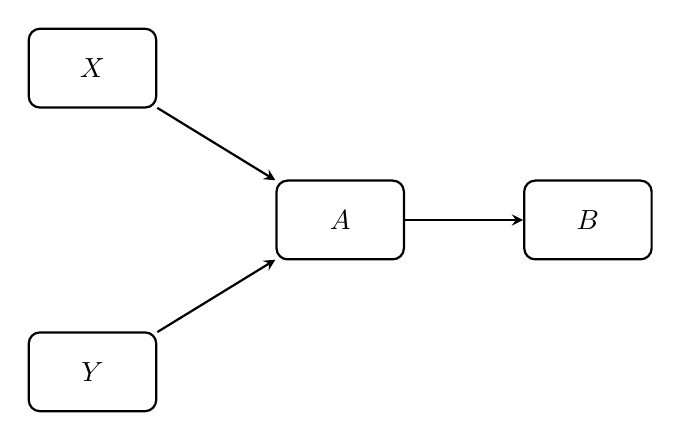
\begin{tikzpicture}[
    scale=0.5,
    ->, % makes edges directed
    >=stealth, % arrow head style
    node distance=0.9cm and 1.5cm, % vertical and horizontal spacing
    thick,
    % Styling for the nodes
    cfgNode/.style={
        rectangle, 
        rounded corners, 
        draw, 
        minimum width=1.618cm, 
        minimum height=1cm, 
        font=\sffamily\bfseries
    }
]

    % Define Nodes
    \node[cfgNode] (A) {$A$};
    \node[cfgNode] (X) [above left=of A] {$X$};
    \node[cfgNode] (Y) [below left=of A] {$Y$};
    \node[cfgNode] (B) [right=of A] {$B$};

    % Draw Edges
    \draw (X) -- (A);
    \draw (Y) -- (A);
    \draw (A) -- (B);

\end{tikzpicture}
    }
    \caption{Example of CFG}
    \label{fig:cfgex1}
\end{figure}

In the example represented in Figure \ref{fig:cfgex1}, under standard AFL++, the transition $A \rightarrow B$ looks identical regardless of the starting block. Under an N-Gram model with $N > 2$, the two possible paths evaluate to distinct hashes, rewarding the fuzzer for discovering a new path.

AFL++ implements this by keeping track of the last $N-1$ previous blocks via an array and injecting instrumentation to modify it at every basic block.

This mode substantially enhances the fuzzer's sensitivity to complex state machines and sequential parsing logic, but it also greatly increases the number of unique identifiers generated.

\subsubsection{Ball-Larus Path Coverage}

Each edge, even when augmented via context sensitivity or N-Gram coverage, inherently remains a decomposition of control flow. However, developers often think about code in terms of logical paths. 

To align the fuzzer's feedback with the true semantic topology of the target program, Ball-Larus Path Coverage treats functions as Directed Acyclic Graphs (DAGs), assigning a unique identifier to every complete acyclic route through a function. 

The Ball-Larus algorithm \cite{ball1996efficient} establishes a method for generating a perfect minimal hash for all paths in an acyclic control graph.

The CFG of a function is transformed into a DAG by removing all loop-back edges. Loops are effectively treated as a single block. Then the graph is traversed from exit back to entry and an integer is assigned to each edge such that the sum of the weights along any path from entry to exit uniquely equates to an integer in the range $[0, NPaths - 1]$ --- with $NPaths$ being the total number of paths in the graph.

During execution, an integer is set to 0 on function entry. As control flows through edges, the weight of each traversed edge is added to the counter. On function exit, the final value of the accumulator uniquely represents the path traversed.

Because of the possible combinatorial explosion in the number of total acyclic paths, AFL++ introduces collapse heuristics. There are various configurations, from strict adherence to the Ball-Larus algorithm to considering only behavioural path divergence, tracked by using a maximum instead of a sum for the number of path counts. 

\subsection{CmpLog Mode}

Standard coverage-guided fuzzers rely on byte-level bit flips and other random mutations to explore an application's state space. While these mutations are effective for broad structural vulnerabilities, they struggle when encountering blocks such as multi-byte comparisons, checksums or parser constraints.

When employing random mutations, the probability of correctly guessing a 64-bit integer is $1$ in $2^{64}$. Solving these constraints has traditionally been done with analysis techniques such as symbolic execution. These approaches, while correct, can be orders of magnitude slower than native execution.

To bypass the costs of symbolic execution, the Redqueen algorithm \cite{aschermann2019redqueen} proposed a solution rooted in the concept of input-to-state correspondence, i.e., the premise that during the execution of a program parts of the input frequently end up in the program state unmodified, or with predictable encoding.

When a highly constrained conditional branch is evaluated, the operands of the comparison instruction or routine often consist of a component derived from the fuzzer's input, an expected constant, or a dynamically generated value.

If a fuzzer can actively monitor and log these operands during execution, it can avoid formally modelling the application's constraints. The fuzzer can directly observe that a specific value is being compared against the execution context. By actively substituting the expected value into the original input the constraint is immediately solved.

AFL++ realises this framework through its CmpLog instrumentation mode. The fuzzing process is divided into two binaries: one for coverage and one with specialized hooks before every memory or string comparison.

When the fuzzer discovers a new path that is heavily constrained or stalling, the fuzzer submits the input to the CmpLog binary. The fuzzer then parses the information given by the additional instrumentation, identifying the values required to traverse previously failed conditional branches.

The Redqueen mutator then attempts to localize these values within the original input --- a process known as \textit{Colourisation}. If the fuzzer can determine which input bytes directly influence comparison operands, it injects the logged target values to satisfy the constraints.

\subsection{MOpt-Adaptive}

Traditionally, stochastic mutations in fuzzers are determined by static probability distributions. This does not take into account the responses of different target applications. For instance, a parser might benefit disproportionately from block splicing, while a cryptographic library might yield more coverage through bit flips.

The MOpt algorithm \cite{lyu2019mopt} models the selection of mutation operators as a Multi-Armed Bandit problem (MAB). The initial implementation utilized Particle Swarm Optimization (PSO) to dynamically update the selection probabilities of mutation operators based on their empirical efficiency during a "pilot" phase.

AFL++ evolved this concept, abandoning PSO in favour of a context-aware MAB framework, stabilised by simulated annealing, exponential decay, and an exploration-exploitation floor. The innovation lies in recognizing that the efficacy of a mutation is not strictly a property of the target application, but rather of the fuzzing context. 

\paragraph{Contextual space} The algorithm partitions the fuzzer's state into a set of discrete contexts, parametrised by two dimensions: 
\begin{itemize}
    \item \textit{Input mode:} Categorising the structure of the seed input; it can be "Generic", "Text" and "Binary".

    \item \textit{Fuzzing mode:} Categorising the objective of the current fuzzing iteration. This can be "Explore", aimed at broad state discovery, and "Exploit", aimed at highly favoured paths.
\end{itemize}
The probability distribution of mutation operators is independently learned and maintained for each context.

\paragraph{Efficacy Measurement} To establish the utility of each mutation operator $i$, MOpt-Adaptive tracks two primary metrics per operator within the active context: "Uses" $U_{i,t}$, representing the number of times an operator has been applied, and "Finds" $F_{i,t}$ representing the number of times the operator successfully contributed to the discovery of a new path.

Both metrics are subject to exponential decay, to prevent historical performance from dominating the future utility. This way, the learned probability distribution remains sensitive to recent features of the application.

There is also a starting static distribution $P$, whose weight decreases linearly over time, down to a minimum floor.

The final probability weight $W_i$ for an operator is a convex combination
\[
    W_i = (1 - \varepsilon) \cdot \frac{F_i}{U_i} + \varepsilon \cdot P_i
\]

This weight is quantised in discrete slots, for faster look-up by using a table. There is an exploration floor; no operator can have fewer than one slot.

The learned distribution is also compared against the predefined static distribution. If the learned array fails to demonstrably outperform the static array's rate of discovery, the fuzzer will naturally fall back to the static distribution.

\subsection{Custom Mutators}

To breach parsing boundaries in complex targets, the mutation engine must have awareness of the input domain. By exposing the custom mutator API, AFL++ allows injecting domain-specific knowledge into the fuzzing loop.

A custom mutator is an external module --- dynamically loaded into the AFL++ process --- that intercepts the mutation phase, allowing for structure-aware alterations. The custom mutator is positioned as the first non-deterministic stage, ensuring that domain-specific mutations are prioritized. It is also possible to enforce the use of custom mutators exclusively, disabling AFL++'s intrinsic mutation stages. This capability is achieved through a series of callbacks managed by the fuzzer process.

By implementing hooks such as \texttt{afl\_custom\_fuzz} and \texttt{afl\_custom\_post\_process}, mutators can translate inputs into intermediate representations, perform targeted structural manipulations (e.g., altering Abstract Syntax Tree nodes), and serialize them back into a valid format. When confronting targets with syntactic constraints, this domain-aware approach ensures that test cases bypass superficial validation layers, allowing the evolutionary algorithm to focus on uncovering vulnerabilities within the deeper logic of the application.


    \chapter{Architecture}
\label{ch:arch}

As shown in Section \ref{ch:afl}, traditional edge coverage relies on a single shared memory bitmap and a hashing function to track execution paths. This approach is highly performant and has led to thousands of bugs being found in recent years \cite{ossfuzz}. 

However, indirect jumps are generally not explicitly tracked and still present a challenge. While these dynamic jumps can be instrumented at compile time, they inherently represent a 1-to-$N$ control-flow mapping, where a single call site may resolve to numerous distinct targets at runtime. 

Attempting to capture this execution within a traditional, fixed-size coverage map significantly increases the probability of collisions. Alternatively, in collision-free modes, it would inflate the size of the map. Either scenario potentially degrades the fuzzer's efficacy. 

In this chapter, we describe our solution, which addresses these problems by introducing a secondary coverage map dedicated exclusively to tracking indirect jumps.

\section{The Indirect Branch Problem}

As detailed in Section \ref{sub:shm}, AFL++ relies on a highly optimised, fixed-size shared memory bitmap (typically 64KB, although resizeable) to track execution paths. 

Indirect branches --- such as function pointers, virtual method dispatches in C++, and complex switch-case statements --- introduce a dynamic $1$-to-$N$ mapping into the CFG. A single indirect call site $A$ does not resolve to a single destination $B$. Instead, depending on the program state, $A$ can transition to one of many targets during execution.

If these indirect branches are instrumented using the standard edge-tracking mechanism, every new target $B_i$ generates a new edge $A \rightarrow B_i$.

\paragraph{The Collision Problem} Mapping these high-volume dynamic edges into the same fixed-size map used for direct edges can significantly increase the overall density of the coverage map. A denser map naturally increases the probability of collisions. 

When a collision occurs, it causes "coverage blindness". The fuzzer might observe an execution that reaches a novel path, but if that edge hashes to a byte already saturated by an indirect branch, the fuzzer will incorrectly assume the path is redundant. Consequently, viable inputs are discarded.

\paragraph{Collision-Free Instrumentation Issues} This problem persists even when utilizing collision-free instrumentation modes, such as LLVM PCGUARD (Section \ref{sub:llvmmode}). These modes achieve zero collisions by assigning a unique ID to every basic block and edge discovered at compile time, sizing the coverage map exactly to the number of known edges.

Because indirect branches resolve at runtime, they circumvent the static counting. If unpredictable dynamic edges were naively introduced into a collision-free map, they would risk breaking the zero-collision guarantee.

Simply extending the coverage map to accommodate all dynamic edges would risk allocating an excessively large map, introducing performance bottlenecks and causing CPU cache thrashing.

\subsection{Requirements for a Solution}

To accurately track indirect branches without polluting the primary coverage map or degrading execution speed, an alternative data structure is required. This structure must satisfy two conflicting constraints: 
\begin{itemize}
    \item \textit{High capacity for dynamic edges:} It must be able to absorb a high volume of unpredictable, runtime-generated edges.

    \item \textit{Strict memory and performance bounds:} It must maintain a small memory footprint to avoid cache thrashing and preserve fuzzing throughput.
\end{itemize}

These requirements point towards a probabilistic data structure capable of tracking set membership with a fixed size and a predictable collision rate --- a role perfectly suited for Bloom filters.

\section{The Secondary Indirect Coverage Map}

To accurately track indirect branches without polluting the primary coverage map or degrading execution speed, an alternative data structure is required. We propose the introduction of a dedicated secondary coverage map for tracking indirect control flow transfers. This architecture aims to resolve the conflicting constraints of maintaining high capacity for dynamic edges while preserving strict memory and performance bounds.

The primary concept relies on utilizing a small Bloom filter for each possible source of an indirect jump: each target reached is then represented by a single bit raised to 1 within the corresponding filter. 

\paragraph{Isolation} We aim to decouple the tracking of indirect branches from the standard coverage map and move this data into an independent shared memory region. Isolation ensures that collisions occurring within the secondary map cannot inadvertently suppress standard edge discovery. 

\paragraph{Collision-Free Identification} For our secondary map, we use a dynamic, sequential "\textit{Guard Array}" architecture. In this model, every indirect branch source in the compiled binary is assigned a guaranteed, sequentially numbered and collision-free slot. 

During the compilation phase, a dedicated ELF section is created, allocating exactly one slot for every \texttt{call} or \texttt{jmp} instruction that resolves dynamically. This approach guarantees that the coverage map possesses a 1-to-1 mapping for the \textit{origins} of all indirect control flow transfers.

\paragraph{Configurable Fidelity} To address the diverse requirements of different target applications, we provide configurable fidelity. The size of the Bloom filter, and consequently the collision tolerance of the secondary map itself, can be tuned. This allows balancing the memory footprint against the granularity of fuzzing feedback.

\section{Compile-Time Instrumentation}

As already detailed (Section \ref{sec:compandinst}), visibility into the target application is achieved through compile-time instrumentation. In our solution, the instrumentation logic is integrated into the LLVM compiler infrastructure, specifically extending the existing LLVM mode's PCGUARD pass. 

The instrumentation process is explicitly designed for indirect branches and consists of three primary phases: target identification, metadata allocation, and callback injection.

\paragraph{Target Identification} The first phase of the instrumentation pass involves traversing the LLVM Intermediate Representation to identify instructions capable of dynamic control flow transfers. 

During the traversal of each basic block, the pass filters the instruction stream to isolate two specific LLVM IR instructions: 
\begin{itemize}
    \item \texttt{IndirectBrInst}: Represents an indirect branch instruction --- e.g., computed \texttt{goto} statements and jump tables.

    \item \texttt{CallInst}: Represents a function call. In this case, the pass further verifies that the target operand is an indirect function pointer call or a virtual method dispatch.
\end{itemize}

To maintain feature parity with the broader AFL++ ecosystem, this identification phase respects the coverage boundaries set for standard edge coverage. Fuzzing campaigns can utilise allowlists and denylists to constrain instrumentation to specific source files or functions.

\paragraph{Guard Array Architecture} Once an indirect instruction has been verified and selected for instrumentation, the compiler allocates a slot to track its execution. To track each indirect branch source, our architecture utilises a metadata structure referred to as "Guard Array".

For every identified indirect instruction, the compiler pass allocates a 32-bit integer slot --- a \texttt{GuardPtr} --- into a dedicated contiguous ELF section named "\texttt{\_\_sancov\_indir\_guard}" (mimicking the operation of PCGUARD mode).

As the compiler processes each translation unit, it continuously appends 32-bit slots into this section. The resulting linked binary will contain a sequential array of uninitialized metadata slots, corresponding one-to-one to every instrumented indirect branch source. At runtime, these slots will be populated with unique sequential identifiers.

\paragraph{Callback Injection} The final phase of static instrumentation involves modifying the target's executable code to report the control flow transition. This requires injecting a C function callback into the LLVM IR.

Modifying the IR of a basic block while actively iterating over its instructions risks invalidating iterators and triggering undefined behaviour within subsequent analysis passes. To circumvent this, a two-phase approach is taken: 
\begin{enumerate}
    \item \textit{Collection Phase:} The pass first traverses the CFG, applying the identification and allowlist logic to build a set of valid targets.

    \item \textit{Mutation Phase:} The pass performs the necessary IR modification on the collected set of targets.
\end{enumerate}

For each target instruction in the mutation set, the compiler injects a call to \texttt{\_\_afl\_trace\_indir} immediately preceding the indirect branch. The callback takes two arguments: the address of the corresponding \texttt{GuardPtr} slot and the target address of the indirect branch, which the program has just evaluated.

\section{Runtime Support}

The runtime component of the indirect coverage system operates alongside the standard compiler runtime and serves as a bridge between the metadata injected by the compiler pass and the actual indirect coverage tracking mechanism of the fuzzer.

Its responsibilities are manifold, spanning from the initialisation of the indirect guard array to the execution of the coverage callback.

\paragraph{Guard Array Initialisation} The lifecycle of the indirect tracking mechanism begins before the target program's \texttt{main} function is executed. The LLVM compiler pass registers a module-level constructor that invokes the initialisation routine.

The objective of this initialisation phase is to transition the guard slots from their uninitialized state into distinct identifiers. The function implements a linear scan across the region of the Guard Array dedicated to the corresponding module. A globally-scoped counter is increased monotonically for each indirect jump source within each module.

If Dynamic Shared Objects (DSOs) are loaded into the process space --- and are instrumented --- their constructors invoke the initialisation function within the bounds of their specific \texttt{\_\_sancov\_indir\_guards} section. The runtime incorporates these new slots into the identifier namespace, ensuring a contiguous ID space across the main executable and all loaded libraries.

Upon completion of the initialisation scan, the final ID value defines the maximum required index for the shared memory map. This value is then communicated to the fuzzer and used to allocate exactly the required memory before the fuzzing loop begins.

\paragraph{Coverage Callback} The core of the tracking mechanism is the callback injected into the IR. This function is executed immediately prior to every indirect control flow transfer and, consequently, is optimised for minimal latency.

The indirect map utilises the unique slot ID as a direct index into the map array. However, a single indirect branch source often dispatches execution to multiple distinct target addresses. To record these diverse destinations, the runtime must efficiently map the target address value to a specific bit within the source's Bloom filter.

To achieve this, each destination is associated with a single bit in the source's Bloom filter using a multiplicative hash function applied to the lower 12 bits of the destination address. The hash result is then truncated to yield an index, and the bit at the corresponding position in the Bloom filter is set to 1.

\section{Execution Evaluation}

The introduction of the secondary indirect coverage map necessitates adjustments to the fuzzer's core heuristics. Specifically, it calls for changes in how the engine evaluates the utility of newly discovered test cases and how the execution queue is managed to prioritise inputs that uncover novel indirect branch targets. Substantial modifications to the execution scheduling algorithm are therefore needed.

\paragraph{Queue Management Integration} The cornerstone of CGF is the ability to recognize when an execution trace reaches novel execution paths. In the standard AFL++ architecture, this is solely governed by comparing the primary edge map against a historical record of all seen edges.

With the introduction of the indirect tracking mechanism, this evaluation phase --- responsible for determining whether a test case should be appended to the fuzzer's queue --- must become dual-faceted. A specialized evaluation function is added to the fuzzer's post-execution routine, performing a comparison between the newly generated indirect map and its historical record.

If novel bits are detected in the secondary map, representing a previously unreached indirect target, the input is immediately qualified as "interesting", similarly to the discovery of a new edge in the standard coverage map. This designation of novelty applies even if the primary edge map yielded no new discoveries. This is crucial as it allows the fuzzer to preserve and explore paths that would otherwise have been obscured.

\paragraph{Seed Scoring} Appending a seed to the queue is only the first step. The scheduler must also determine the quality of the input. AFL++'s scheduling algorithm relies on the concept of "favoured" entries, which are selected more frequently for mutation. To minimise corpus size while maintaining maximum coverage, the fuzzer prioritises the fastest and smallest inputs that cover each known edge (as seen in Section \ref{subsec:qandsched}).

To mirror the standard logic for the indirect map, a secondary array of top-rated entries is introduced, specifically for entries valuable in terms of bits set in the secondary map.

The fuzzer evaluates the current test case's characteristics: 
\begin{itemize}
    \item Whether the test case is the very first to trigger a specific bit in the secondary map.

    \item Whether the test case triggers an already known target but represents a more performant execution path than the previously recorded best input for that target.
\end{itemize}
In either case, the input captures the "top-rated" slot for that specific indirect bit. This strict preservation logic ensures the engine explicitly retains the most efficient inputs required to reach every discovered indirect destination, forming a solid baseline for subsequent mutation cycles.

\paragraph{Performance Multipliers} When selecting a test case from the queue to undergo mutation, the fuzzer calculates a "performance score", which determines the intensity and duration of the fuzzing cycle allocated to that seed. Higher scores translate to more mutation cycles. 

The calculation of this score has been augmented to incorporate the density of the indirect coverage map. Testcases that successfully uncover a significant number of paths containing indirect branches are awarded higher performance multipliers. This heuristic guides the mutation engine to focus its computational resources on inputs that have already demonstrated the capability to explore more traditionally obscure areas of the application's CFG. 

\paragraph{Trace Verification and Execution Checksums} To maintain the integrity of the fuzzing state, AFL++ validates execution traces to ensure determinism and identify stability issues. A non-deterministic path can degrade the fuzzer's efficiency and introduce noise into the feedback loop. 

During operations such as test case calibration and trace minimisation, the fuzzer computes checksums of the coverage bitmap to verify stability. The checksumming routines have been modified to incorporate the secondary map.

The fuzzer now computes a combined checksum representing the state of both the primary edge map and the secondary indirect map. If the indirect map diverges between identical runs, the fuzzer's stability metrics will correctly flag the execution as variable. This validation ensures that the fuzzer does not erroneously optimise or prioritise inputs based on unstable indirect control flow, thereby maintaining the fidelity of the overall fuzzing campaign.
    
    \chapter{Implementation}
\label{ch:impl}

This chapter details the modifications made within AFL++ to support the architecture described in the previous chapter. Implementing these features requires alterations across multiple independent subsystems, spanning the fuzzer's core orchestrator, the LLVM compile-time instrumentation, and the runtime support libraries.

\section{Data Structures and Core Types}

To establish the tracking mechanism, several foundational data types and state variables had to be introduced.

These modifications are all contained within several of the project's main headers: \texttt{include/types.h}, \texttt{include/afl-fuzz.h}, \texttt{include/sharedmem.h}, and \texttt{include/config.h}.

\subsubsection{Configurable Slot Types}

To provide tunable fidelity, the width of the bitfield used to track distinct targets originating from a single indirect source --- i.e., the size of each Bloom filter --- is made configurable via the compiler preprocessor. This configuration is codified by the \texttt{INDIR\_SLOT\_SIZE} compile-time macro. It defaults to a size of 64.

The header \texttt{types.h} subsequently constructs the \texttt{indir\_slot\_t} alias utilising preprocessor conditionals based on the value of the aforementioned macro:
\begin{itemize}
    \item \texttt{INDIR\_SLOT\_SIZE == 32}: \texttt{indir\_slot\_t} resolves to \texttt{uint32\_t}.
    
    \item \texttt{INDIR\_SLOT\_SIZE == 64}: \texttt{indir\_slot\_t} resolves to \texttt{uint64\_t}.
    
    \item \texttt{INDIR\_SLOT\_SIZE == 128}: \texttt{indir\_slot\_t} resolves to \texttt{unsigned \_\_int128}.
\end{itemize}

By exclusively employing \texttt{indir\_slot\_t} across the fuzzer, the entire architecture scales to accommodate the designated slot width without requiring localised code modifications. This ensures type safety and prevents hardcoded integer sizes throughout the codebase.

Alongside the type alias, the header defines the \texttt{INDIR\_BIT\_SHIFT} constant, representing the base 2 logarithm of the slot size --- e.g., 6 for 64-bit. This is used inside the callback to construct a bitmask used for the modulo reduction of the hashed target address.

\subsubsection{Fuzzer State Encapsulation}

The fuzzer's context is entirely encapsulated within the \texttt{afl\_state\_t} structure. This structure was extended to manage the new coverage domain. Additions include: 
\begin{itemize}
    \item \texttt{indir\_map}: A pointer to the shared memory region populated by the target binary.
    
    \item \texttt{indir\_virgin\_bits}: A persistent array storing the cumulative history of all discovered indirect path transitions across the entire campaign. This is the reference used to evaluate novelty after executions.
    
    \item \textit{Top Entries Structures}: Additional arrays were introduced to track and retain the inputs that maximise specific bit transitions within the indirect map, mirroring the behaviour of the primary map's top-rating system.
\end{itemize}

\subsubsection{Shared Memory IPC Metadata}

The \texttt{sharedmem\_t} structure maintains the IPC primitives and metadata required to manage the shared memory segments. The structure was extended with: 
\begin{itemize}
    \item \textbf{\texttt{indir\_map\_size}}: An integer recording the currently allocated size of the secondary shared memory segment. This is updated whenever the fuzzer issues a reallocation based on forkserver feedback.
    
    \item \textbf{\texttt{indir\_shm\_id}}: The active System V IPC identifier associated with the allocated \texttt{indir\_map}.
\end{itemize}

\section{LLVM Pass and Instrumentation}

Modifications to the \texttt{SanitizerCoveragePCGUARD} pass serve to statically identify indirect control flow transfers and inject the tracking metadata and runtime callbacks. The core of the indirect jump tracking mechanism relies on targeted compile-time modifications.

\subsubsection{The Guard Array Architecture}

When the pass executes, it identifies all valid indirect branches within a function. For each function containing at least one indirect branch or call, the pass generates a local array of integers with a length equal to the number of indirect instructions identified.

The compiler assigns a specific section attribute to these arrays: \texttt{\_\_sancov\_indir\_guards}. The linker guarantees that all such arrays, scattered across different translation units, are concatenated into a contiguous region within the final ELF binary.

For each instruction, the compiler calculates the address of its corresponding element within the guard array, yielding a value that represents the memory location of the slot assigned to that instruction, which enables guard pointer resolution at runtime.

\subsubsection{Instruction Injection}

The primary objective of the instrumentation pass is to inject the callback \texttt{\_\_afl\_trace\_indir} immediately before the execution of any indirect branch. A new, separate routine is added to manage this modification in a two-phase operation: first, all relevant \texttt{IndirectBrInst} and \texttt{CallBase} instructions are aggregated; then, the pass allocates the corresponding guard slot and prepares to inject the callback.

During callback injection, the compiler utilises an \texttt{IRBuilder} immediately before the target instruction, creating the callback with the following signature:
\begin{minted}{c}
void __afl_trace_indir(uint32_t *guard, uintptr_t target_addr);
\end{minted}

The pass provides the following arguments: the pointer to the instruction's 32-bit slot in the \texttt{\_\_sancov\_indir\_guards} section and the resolved destination address of the \texttt{jump} or \texttt{call}.

The LLVM pass operates independently of the \texttt{INDIR\_SLOT\_SIZE} macro; its sole responsibility is to pass the pointer to the 32-bit sequential ID. Interpretation and scaling based on slot width are handled entirely within the compiler runtime.

\section{Compiler-RT}

The runtime library (\texttt{instrumentation/afl-compiler-rt.o.c}) acts as a layer between the LLVM-generated structures and the dynamic coverage tracking of the fuzzer. Among its responsibilities are the initialisation of the guard array, the calculation of the required shared memory footprint, and the execution of the callback.

\subsubsection{Guard Array Initialisation}

The execution lifecycle of the secondary coverage map mechanism starts prior to the execution of \texttt{main}, with the module-level constructor:
\begin{minted}{c}
__afl_indir_trace_pc_guard_init(uint32_t *start, uint32_t *stop)
\end{minted}

The linker guarantees that \texttt{start} and \texttt{stop} represent the boundaries of the contiguous \texttt{\_\_sancov\_indir\_guards} section containing the guard slots for the module in question.

The primary job of this initialisation function is to assign unique identifiers to each slot. Using an atomic counter (\texttt{\_\_afl\_indir\_final\_loc}), it scans the region \texttt{[start, stop)} and, for each uninitialised guard slot, writes the current value of the counter and increments it.

\subsubsection{Dynamic Map Sizing}

Upon completion of the guard initialisation scan, the required map dimension is computed as \texttt{\_\_afl\_indir\_final\_loc + 1}. This is the exact dimension needed for all sources found during initialisation and is assigned to the state variable \texttt{\_\_afl\_indir\_map\_size}. 

If the mapped shared memory segment provisioned by the fuzzer is smaller than the required value, the runtime redirects the \texttt{\_\_afl\_indir\_map} to a dummy map, which acts as a safe sink to prevent out-of-bounds writes. All subsequent coverage updates are absorbed until the fuzzer provisions an adequately sized shared memory region.

\subsubsection{The Coverage Callback}

The core of the computations for the tracking mechanism is the \texttt{\_\_afl\_trace\_indir} callback, executed immediately prior to every indirect control flow transfer. To minimise runtime overhead, several performance optimisations are applied. 

The callback immediately exits if the ID referenced by the guard pointer is 0 --- indicating a non-instrumented DSO --- or if the \texttt{\_\_afl\_indir\_ptr} is invalid --- either because it is 0 or because it points to the dummy map.

The callback then utilises the retrieved ID as an index into the \texttt{\_\_afl\_indir\_map} array. However, to track multiple targets per indirect source, the target address undergoes a multiplicative hash. The result is masked using \texttt{INDIR\_BIT\_SHIFT} to compute a safe bit index. The index is then used to set the corresponding bit within the designated slot of the shared memory map, recording the traversed edge.

Fibonacci hashing is used as it ensures a highly uniform distribution of values across the table \cite{knuth1998art3}, while also being computationally inexpensive; it can be calculated in a single clock cycle.

The full callback definition is provided inside Appendix \ref{app:fuzzr}. 

\section{Forkserver and IPC}

Low-latency communication between the fuzzer and the target process is fundamental for the dynamic sizing of the map. The required map size depends on the target binary's structure and complexity, so the fuzzer needs to determine the appropriate size, which is only known after initialisation. This dependency is resolved through some modifications to the AFL++ forkserver handshake protocol.

\subsubsection{The \texttt{FS\_NEW\_OPT\_INDIR\_MAPSIZE} Signal Protocol}
\label{subsub:signalprot}

The AFL++ forkserver uses a pair of pipes to mediate the execution lifecycle of the target binary. During the initial handshake sequence, the instrumented binary communicates its configuration to the fuzzer by writing a bitfield of operational flags to the status pipe.

To facilitate the transmission of the calculated indirect map size, a new flag \texttt{FS\_NEW\_OPT\_INDIR\_MAPSIZE} is defined within the shared header \texttt{include/forkserver.h}.

\paragraph{Target-Side Transmission} After calculating the map size, the compiler runtime executes the initial forkserver handshake. It asserts the \texttt{FS\_NEW\_OPT\_INDIR\_MAPSIZE} bit within the status payload. Following the transmission of the primary status flags, the runtime executes an out-of-bounds (OOB) write to the status pipe, transmitting the 32-bit unsigned integer value of the map size. This OOB data transmission ensures backward compatibility; older fuzzers unequipped to parse the new flag will just ignore the trailing bytes.

\paragraph{Fuzzer-Side Reception} In the routine to start the forkserver, the fuzzer process enters a read state, awaiting the initial status payload. Upon detecting the \texttt{FS\_NEW\_OPT\_INDIR\_MAPSIZE} flag in the status bitfield, the fuzzer transitions to a secondary read state to extract the transmitted four bytes from the status pipe.

The received integer value is assigned to the indirect map size value in the forkserver state (\texttt{fsrv->indir\_map\_size}). To prevent unaligned memory faults during bitmap evaluation, the fuzzer rounds up the received memory size to the nearest multiple of 64 bytes.

\subsubsection{Environment Variable Propagation}

While the forkserver pipe handles the direct transmission of the map size, the fuzzer must manage the communication of the shared memory location to the spawned target processes. Similarly to the standard coverage map, this is achieved through environment variable injection.

When the fuzzer allocates the secondary memory region, it constructs and exports the \texttt{\_\_AFL\_INDIR\_SHM\_ID} environment variable string. When using POSIX shared memory, the variable contains the virtual path identifier used to open the shared memory object. For consistency, the variable \texttt{AFL\_INDIR\_MAP\_SIZE} is also exported, after being set to the rounded-up size calculated during the handshake.

During the actual fuzzing loop, when the forkserver clones the target process, these environment variables are inherited by the child process. The runtime component parses them to attach to the correct shared memory segment and verify the size value of the mapped region.

\section{Fuzzer Core Orchestration}

The modifications to the core of the fuzzer orchestration, spanning \texttt{src/afl-fuzz.c}, \texttt{src/afl-sharedmem.c}, and \texttt{src/afl-fuzz-bitmap.c}, focus on the allocation, reallocation, and continuous analysis of the \texttt{indir\_map}.

\subsubsection{Dynamic Memory Reallocation}

To determine the size of the secondary map, a probe-and-resize strategy is used.

\begin{enumerate}
    \item \textit{Initial Provisioning:} At startup, the fuzzer provides a dummy shared memory segment using the \texttt{DEFAULT\_INDIR\_SHMEM\_SIZE} macro.
    
    \item \textit{Handshake Resolution:} During the forkserver start sequence, the true required size is transmitted.
    
    \item \textit{Dynamic Reallocation:} If the reported target size differs from the currently allocated size, the fuzzer initiates a reallocation sequence. It invokes the shared memory de-initialisation function on the existing indirect map to unmap the memory, which is then reinitialised to a correctly sized contiguous block.
\end{enumerate}

\paragraph{Preserving Virgin Bits} During reallocation, the fuzzer must preserve accumulated coverage data, stored in the indirect virgin map. A naive reallocation would cause the fuzzer to forget previously explored paths.

To solve this, the implementation uses \texttt{ck\_realloc} to expand the indirect virgin map allocation. The newly appended tail region of the array --- i.e., the previously unmapped guard slots --- must be initialised to \texttt{0xFF}, signifying "unseen" transitions, while keeping intact the lower indices.

%The full reallocation logic is included in Appendix \ref{app:fuzzr}.

\subsubsection{Vectorised Bitmap Iteration}

The performance of the fuzzer depends on the efficiency of evaluating the coverage map after every execution run.

Dedicated functions have been added to iterate over the map, with the size being dictated by the state of the fuzzer process, and determine whether novelty was discovered during execution or to count the number of bits set in the map for reporting purposes.

The iteration uses vectorised 64-bit integer chunking, similarly to the standard coverage map, to improve performance and maintain a high throughput. Each 64-bit comparison requires a single clock cycle, as would comparisons of smaller sizes. Without the aforementioned alignment padding (Section \ref{subsub:signalprot}) applied to the map size, the iteration might fail or skip the trailing unaligned bytes.

\section{Queue Management and Seed Scoring}

The integration of the secondary coverage map dictates the need for adjustments to the fuzzer's core heuristics, altering how test cases are evaluated. The scheduling algorithms (\texttt{src/afl-fuzz-queue.c}, \texttt{src/afl-fuzz-run.c}) were updated to ensure that the fuzzer actively prioritises inputs that uncover new indirect execution paths.

\subsubsection{Top Rated Seeds and Queue Culling}

Mirroring the standard coverage map's scoring system, the fuzzer evaluates executions against a \texttt{top\_rated\_indir} array. For each active bit in the \texttt{indir\_map}, the fuzzer explicitly preserves the smallest and fastest test case required to trigger each specific indirect target.

During the \texttt{cull\_queue} routine, AFL++ iterates over the \texttt{indir\_top\_rated} array to select favoured seeds. Test cases that hit indirect paths not covered by other favoured seeds are explicitly marked as \texttt{favored}, prioritising execution during the fuzzing loop. The map representation is never minimised as it is already "minimal" by design.

\subsubsection{Execution Verification and Checksums}

To maintain the integrity of the fuzzing state, AFL++ validates execution traces to ensure determinism. The checksum algorithms and trace validations executed during calibration have been modified to compute and verify a second hash. A new checksum for the indirect map is calculated and verified:
\begin{minted}{c}
if (unlikely(q->exec_cksum != cksum || 
    (afl->shm.indir_mode && q->indir_cksum != indir_cksum))) 
\end{minted}
This exposes variable execution states, allowing the fuzzer's stability metric to correctly flag the trace as variable.

\subsubsection{Queue Additions and Performance Multipliers}

Upon run completion, the state of the secondary map is evaluated against the historical trace of seen bits. If new indirect targets are found, the input is immediately appended to the active queue. This input is explicitly marked as finding new coverage, even if the primary map reported no discoveries.

When calculating the performance score of a seed, the fuzzer also takes into account the density of the secondary map. A higher number of indirect branches triggered results in higher performance multipliers. Furthermore, performance score bonuses are awarded to inputs that cover more than the average number of indirect targets across all seeds.
    
    \chapter{Evaluation}
\label{ch:eval}

This chapter presents an empirical evaluation of the proposed architecture. The primary objective is to assess whether tracking indirect control flow through a secondary coverage map yields tangible improvements in path discovery and overall fuzzing efficacy when compared to standard techniques.

To evaluate the system, we compare the baseline AFL++ fuzzer against our modified architecture across a diverse set of real-world benchmarks, chosen for their varying levels of reliance on indirect branching. The evaluation is structured to address the core performance and coverage metrics that define a fuzzer's success.

\section{Experimental Setup}

This section outlines the hardware environment, the selected target programs, the fuzzer configurations under test, and all other parameters concerning the fuzzing campaign.

\subsection{Methodology and Environment}

All fuzzing campaigns were executed on a dedicated server running Ubuntu 24.04.4 LTS. The machine is equipped with a 64-core Intel Xeon Silver 4316 processor operating at 2.30GHz and 64GB of RAM.

To ensure the evaluation reflects real-world conditions, we selected a diverse set of targets taken from the FuzzBench repository, alongside a Ruby parser. The selected benchmarks are: 
\begin{itemize}
    \item \texttt{libxslt}
    
    \item \texttt{openssl}
    
    \item \texttt{sqlite3}
    
    \item \texttt{systemd-link-parser}
    
    \item \texttt{mruby}
\end{itemize}

These targets were deliberately chosen for their reliance on complex parsing logic and frequent use of indirect branches, which makes them ideal candidates for testing the efficacy of the proposed indirect coverage map. The inclusion of \texttt{mruby}, a lightweight Ruby implementation, further stresses the fuzzer's ability to navigate the complex indirect jumps typically found in interpreters --- e.g., in the dispatch loop.

\paragraph{Fuzzer Configurations} The analysis was conducted by comparing the standard configuration of AFL++ and our custom AFL++ architecture. The latter was tested in three different configurations: with slot sizes of 32, 64, and 128 bits.

All targets were compiled with the \texttt{afl-clang-fast} wrapper, ensuring all performance or coverage deviations can be attributed to the newly introduced mechanism.

\paragraph{Campaign Parameters} Fuzzing is inherently stochastic; therefore, single-run measurements are insufficient for drawing robust conclusions. For our campaign, each target version was fuzzed for 24 hours, restricted to a single core per run. To ensure statistical significance and account for randomness, we performed 5 independent trials per target version.

\section{Edge Coverage and Path Discovery}

This section presents the primary metrics used to evaluate the efficiency of the proposed modifications: total region coverage and queue size. We compare the standard AFL++ baseline with the modified versions across all targets.

\subsubsection{Total Edge Coverage}

The primary indicator of a fuzzer's overall success is the total number of unique code regions discovered over time. To measure this, coverage analysis was performed using \texttt{llvm-cov}. For each campaign, we gathered the inputs saved in the fuzzer's queue and replayed them against an \texttt{llvm-cov}-instrumented binary. By ordering the queue inputs by creation timestamp, we computed the cumulative region coverage over the 24-hour fuzzing campaigns.

The following plots illustrate the average region coverage growth for each benchmark over 24 hours.

% --- PAGE 1 ---
\begin{figure}[htbp]
    \centering

    \begin{subfigure}{\textwidth}
        \centering
        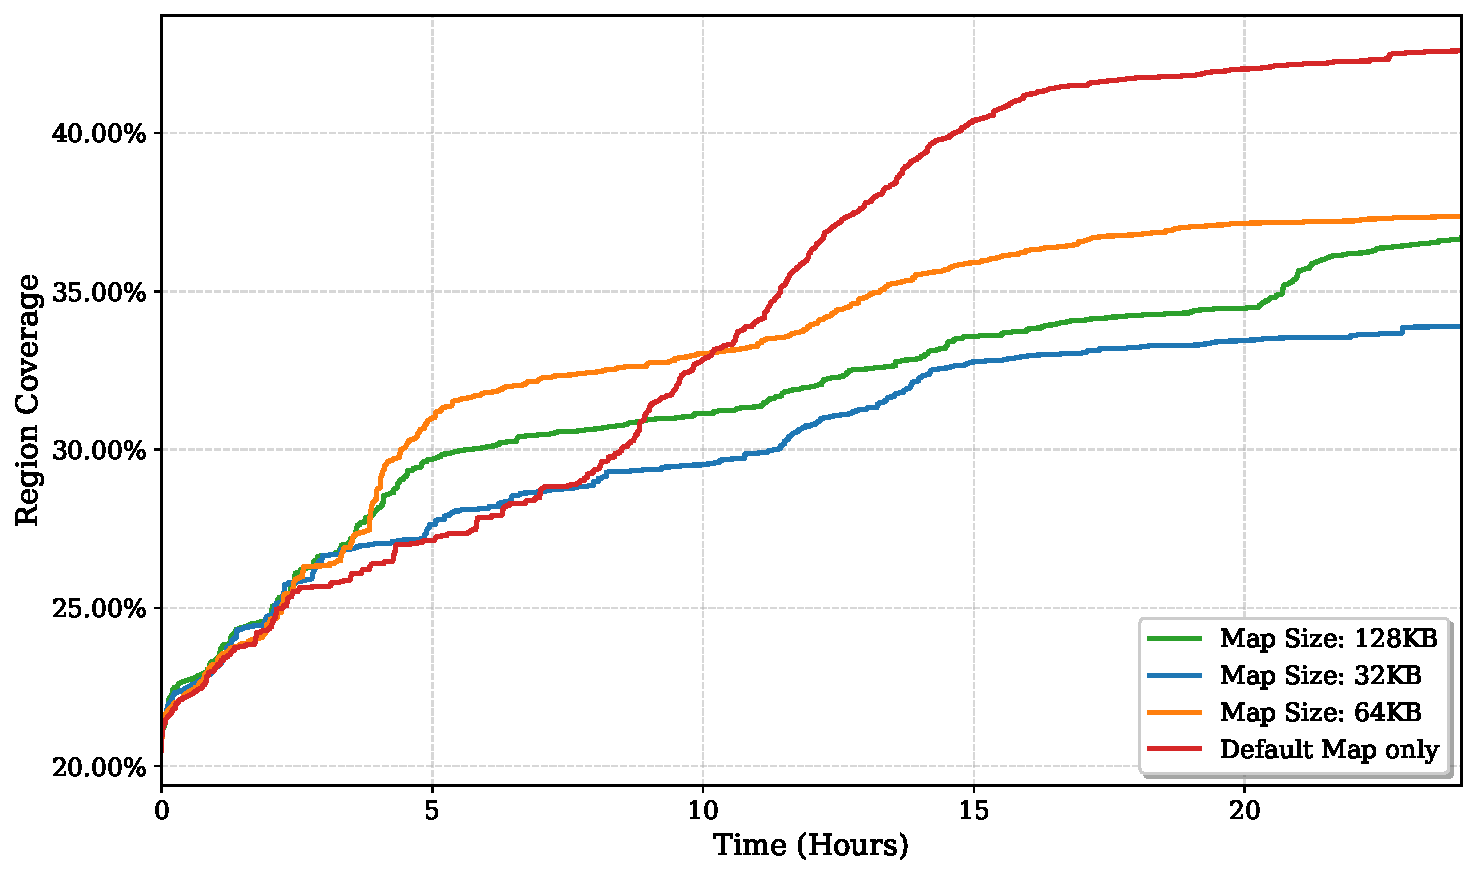
\includegraphics[width=0.85\linewidth]{imgs/eval/coverage_plot_mruby.pdf}
        \caption{mruby}
        \label{fig:plot_mruby}
    \end{subfigure}

    \vspace{2em} 

    \begin{subfigure}{\textwidth}
        \centering
        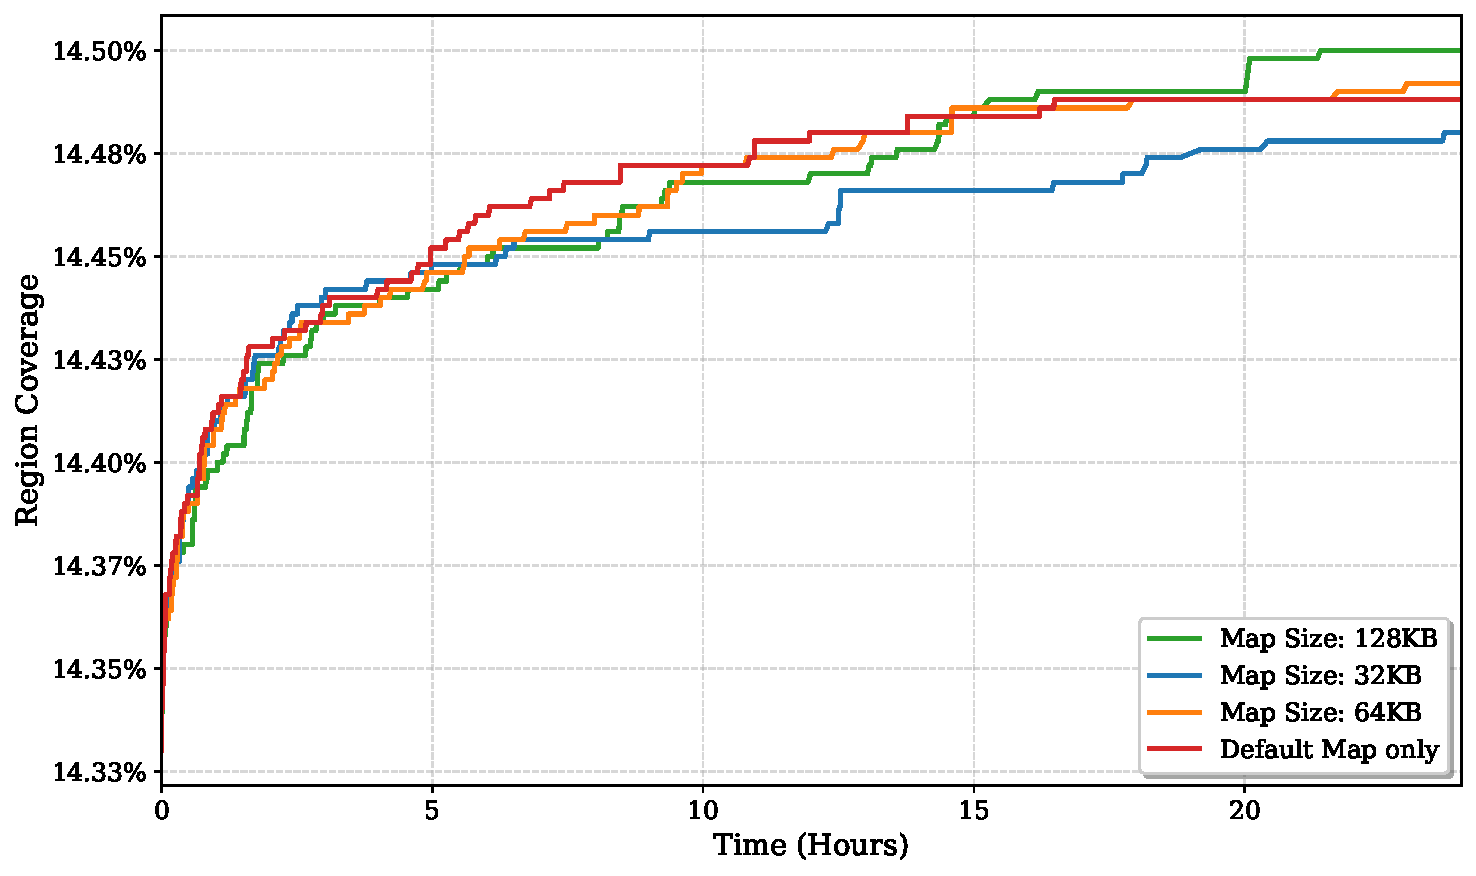
\includegraphics[width=0.85\linewidth]{imgs/eval/coverage_plot_openssl.pdf}
        \caption{OpenSSL}
        \label{fig:plot_openssl}
    \end{subfigure}

    \caption{Coverage over 24 hours for various fuzzing targets (Part 1).}
\end{figure}

% --- PAGE 2 OF THE FIGURE ---
\begin{figure}[htbp]
    \ContinuedFloat % This keeps the figure number the same
    \centering

    \begin{subfigure}{\textwidth}
        \centering
        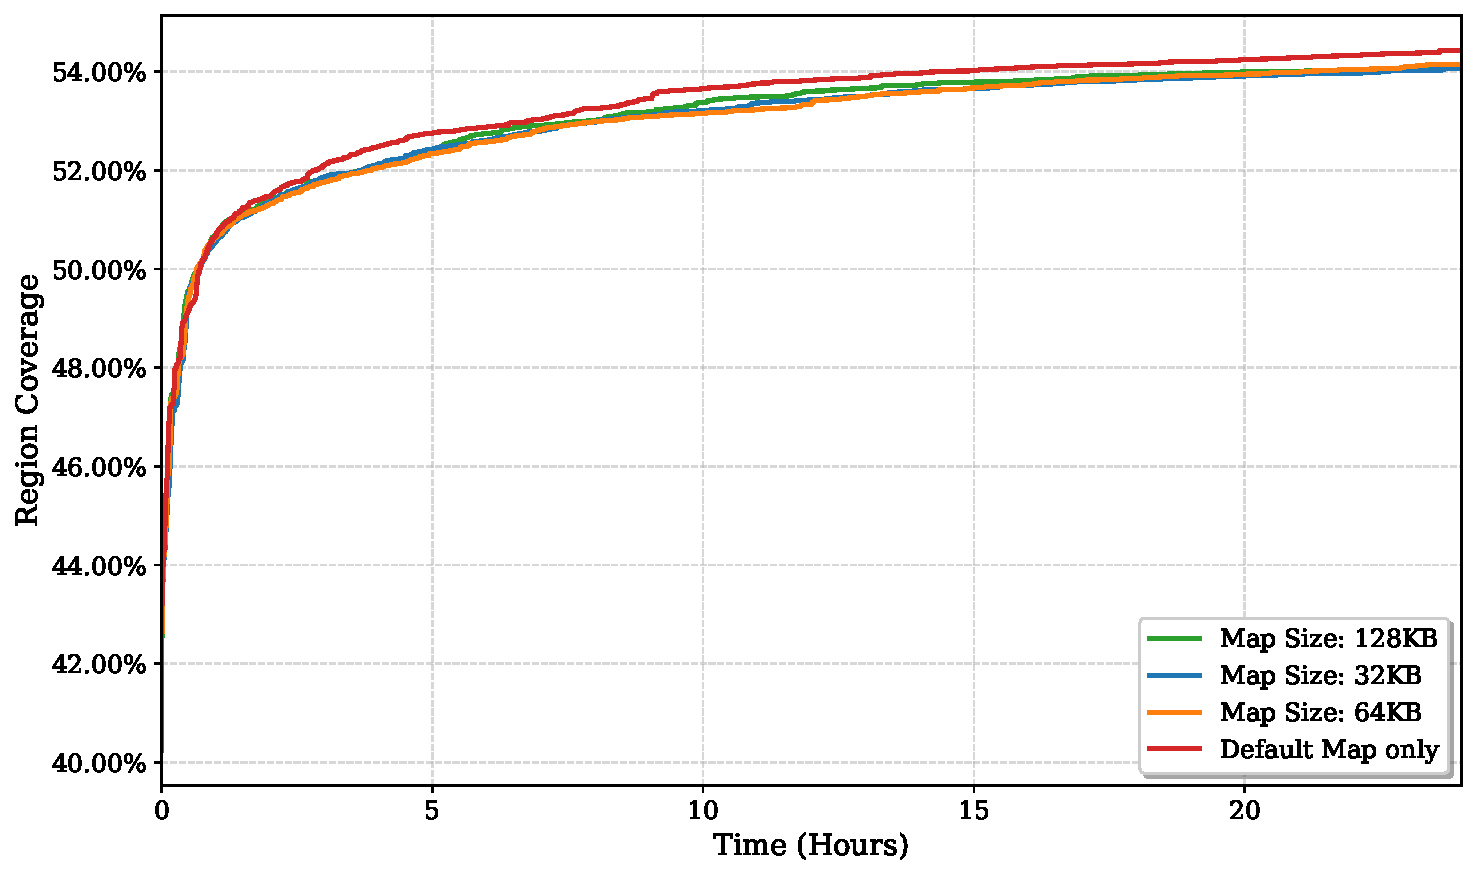
\includegraphics[width=0.85\linewidth]{imgs/eval/coverage_plot_libxslt.pdf}
        \caption{libxslt}
        \label{fig:plot_libxslt}
    \end{subfigure}
    
    \vspace{2em}

    \begin{subfigure}{\textwidth}
        \centering
        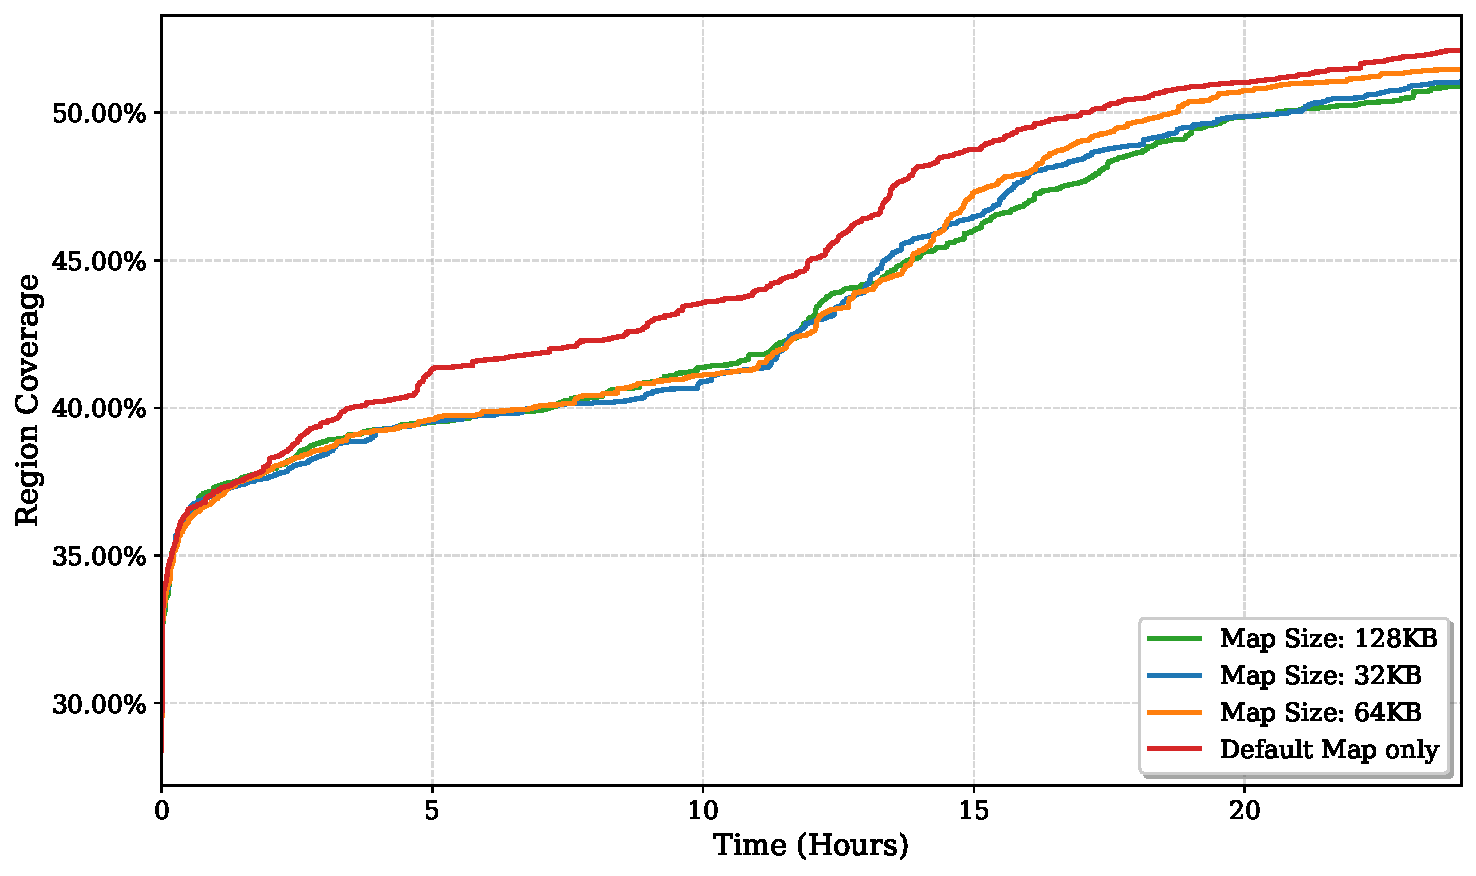
\includegraphics[width=0.85\linewidth]{imgs/eval/coverage_plot_sqlite3.pdf}
        \caption{SQLite3}
        \label{fig:plot_sqlite3}
    \end{subfigure}
    
    \caption{Coverage over 24 hours for various fuzzing targets (Part 2).}
\end{figure}


\begin{figure}[htbp]
    \ContinuedFloat % This keeps the figure number the same
    \centering

    \begin{subfigure}{\textwidth}
        \centering
        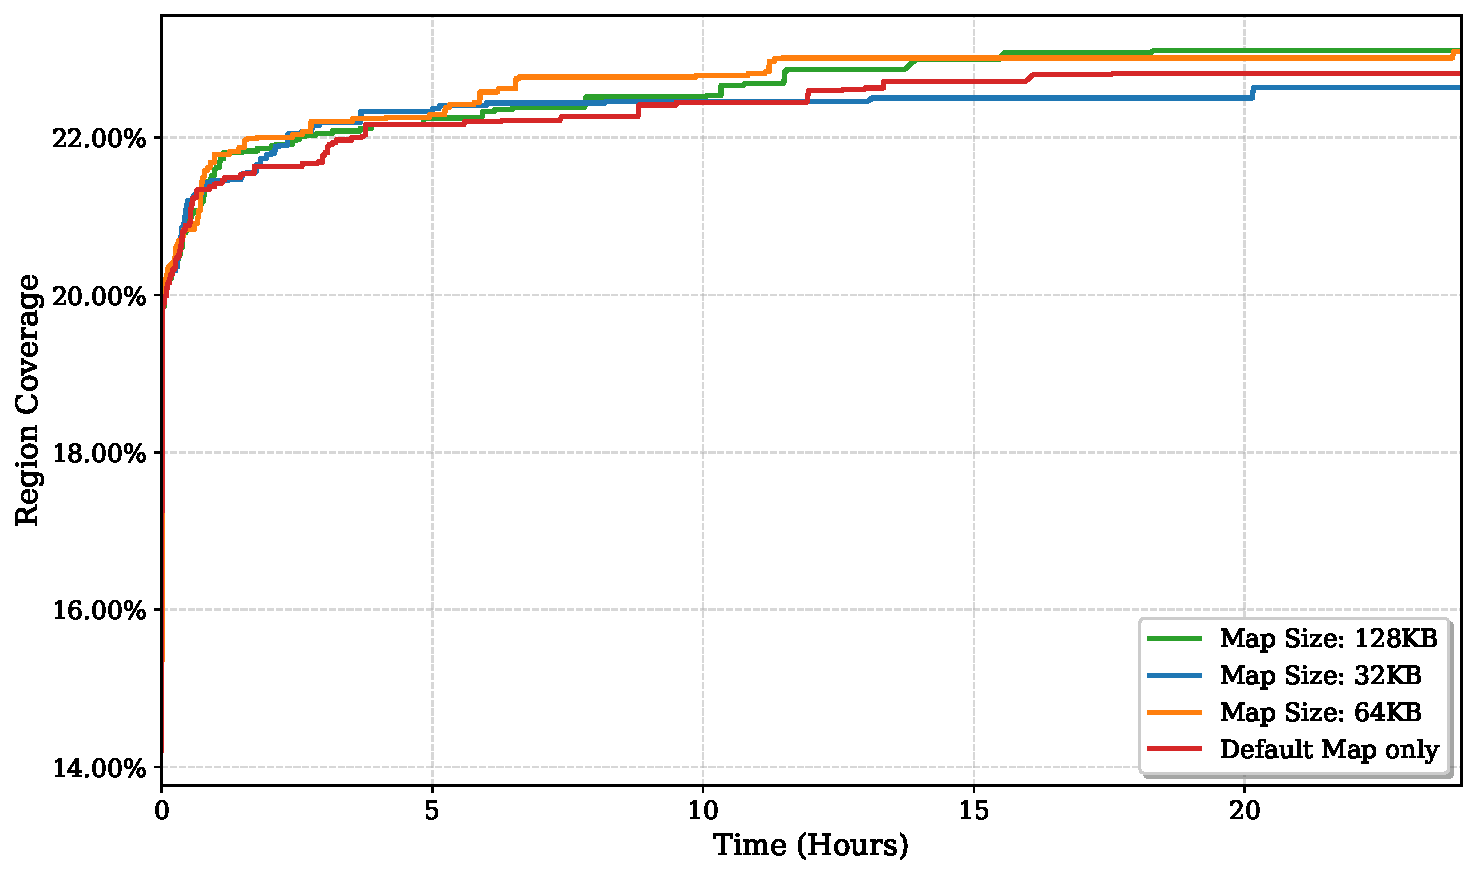
\includegraphics[width=0.85\linewidth]{imgs/eval/coverage_plot_systemd.pdf}
        \caption{systemd}
        \label{fig:plot_systemd}
    \end{subfigure}

    \caption{Coverage over 24 hours for various fuzzing targets (Part 3).}
    \label{fig:cov_plots} % The main label 
\end{figure}

\newpage

The results reveal that, across all tested benchmarks, the modified fuzzer configurations did not achieve a breakthrough in path discovery. In fact, the baseline AFL++ consistently performed either on par with or slightly better than the modified versions in terms of discovered regions within the given time frame.

Table \ref{tab:region_coverage} shows the cumulative region coverage at the end of the campaign for each target and configuration.

\begin{table}[htbp]
    \centering
    \begin{tabular}{@{}l cccc @{}}
        \toprule
        & \multicolumn{4}{c}{\textbf{Fuzzer Configuration}} \\
        \cmidrule(l){2-5}
        \textbf{Target} & \textbf{32 bit} & \textbf{64 bit} & \textbf{128 bit} & \textbf{Default} \\
        \midrule
        \textbf{libxslt} & 54.06\% & 54.14\% & 54.06\% & 54.43\% \\
        \textbf{mruby}   & 33.89\% & 37.36\% & 36.70\% & 42.61\% \\
        \textbf{openssl} & 14.48\% & 14.49\% & 14.50\% & 14.48\% \\
        \textbf{sqlite3} & 51.04\% & 51.46\% & 50.88\% & 52.11\% \\
        \textbf{systemd} & 23.10\% & 23.57\% & 23.58\% & 23.29\% \\
        \bottomrule
    \end{tabular}
    \caption{Average Region Coverage after 24 Hours}
    \label{tab:region_coverage}
\end{table}

Variations across configurations are generally minor. The 32-bit configuration more consistently results in the lowest region coverage among the modified setups. This can be attributed to a higher probability of collisions within the smaller Bloom filter, which saturates prematurely. The 64-bit and 128-bit configurations performed marginally better; however, they consistently failed to outperform the vanilla AFL++ baseline.

\subsubsection{Corpus Size}

The fuzzer's corpus (or queue) size indicates the number of unique "interesting" test cases retained during the campaign. A steadily growing queue typically indicates the continuous discovery of new paths.

The final queue sizes at the end of the campaigns are summarised in Table \ref{tab:corpus_sizes}.

\begin{table}[htbp]
\centering
\begin{tabular}{lrrrr}
\toprule
& \multicolumn{4}{c}{\textbf{Fuzzer Configuration}} \\
\cmidrule(l){2-5}
\textbf{Target} & \textbf{32 bit} & \textbf{64 bit} & \textbf{128 bit} & \textbf{Default} \\
\midrule
\textbf{libxslt} & 17,509.20 & 17,751.60 & 17,504.60 & 18,127.00 \\
\textbf{mruby}   & 5,881.40  & 8,414.80  & 7,381.00  & 11,122.80 \\
\textbf{openssl} & 2,909.20  & 2,916.40  & 2,935.80  & 2,931.00 \\
\textbf{sqlite3} & 11,054.40 & 10,761.80 & 9,875.80  & 13,026.00 \\
\textbf{systemd} & 2,173.40  & 2,125.80  & 2,171.00  & 2,261.00 \\
\bottomrule
\end{tabular}
\caption{Average Corpus Sizes after 24 Hours}
\label{tab:corpus_sizes}
\end{table}

The queue size dynamics closely mirror the region coverage data. Across all targets, the baseline AFL++ and the modified configurations maintain similar queue sizes.

This strongly implies that the indirect map rarely triggered additional seed saves. When an indirect branch was resolved dynamically, the input was almost always already flagged as "interesting" by the primary coverage map.

\section{Performance Overhead}

While the primary goal of the additional coverage map is to increase path discovery, any added instrumentation inherently risks reducing the execution throughput. A significant drop in executions per second (exec/s) can offset the benefits of better feedback. This section evaluates the computational penalty introduced by our architecture.

\subsubsection{Execution Throughput}

To assess the impact, we compared the average executions per second across all campaigns for all tested configurations.

\begin{table}[htbp]
\centering
\begin{tabular}{lrrrrr}
\toprule
& \multicolumn{4}{c}{\textbf{Fuzzer Configuration}} \\
\cmidrule(l){2-5}
\textbf{Target} & \textbf{32 bit} & \textbf{64 bit} & \textbf{128 bit} & \textbf{Default} & \textbf{Overhead} \\
\midrule
\textbf{libxslt} & 586.28 & 644.88 & 587.78 & 698.71 & +13.22\% \\ 
\textbf{mruby} & 70.10 & 75.42 & 74.82 & 79.10 & +7.15\% \\ 
\textbf{openssl} & 2732.29 & 2610.04 & 2836.24 & 3644.51 & +25.2\% \\ 
\textbf{sqlite3} & 407.75 & 424.23 & 381.44 & 452.38 & +10.59\% \\ 
\textbf{systemd} & 115.13 & 110.06 & 111.76 & 110.53 & -1.62\% \\ 
\bottomrule
\end{tabular}
\caption{Average Execs Per Second and Resulting Overhead}
\label{tab:exec_overhead}
\end{table}

Table \ref{tab:exec_overhead} shows the average execution speeds and average overhead across all configurations. 

The data indicates that the secondary map, along with all the necessary mechanisms, introduces a measurable execution penalty that varies heavily by target. Across the benchmarks, the modified fuzzer experienced overhead ranging from $7\%$ to over $25\%$ --- with the anomaly of \texttt{systemd}, which can be attributed to environmental noise and statistical margin of error. 

Targets with particularly high densities of indirect branches exhibited the worst degradation. Furthermore, a significant proportion of the overhead resides in the post-execution phase, meaning that targets with higher absolute numbers of executions per second seem to suffer greater proportional degradation.

Some of the overhead is attributable to the injection of a callback, as the routine to call a function is computationally expensive. This could be mitigated in the future by injecting LLVM IR directly instead of relying on a function call.

\section{Analysis of Results}

As established in the previous sections, the failure of the modified fuzzer to outperform the baseline cannot be solely attributed to performance overhead. The lack of improvement, despite the functional mechanism, points to structural and theoretical limitations in how fuzzers interact with indirect control flow. This section details potential reasons why the indirect coverage map did not yield the expected improvements.

\subsection{Redundancy with the Primary Edge Map}

The primary reason why the modified architecture behaves similarly to standard AFL++ is that the new map provides almost entirely redundant feedback for fully instrumented targets. 

When an indirect jump dynamically resolves to a new target block, there will almost certainly be some new direct edges to be tracked by the standard coverage map. The injected callback is invoked immediately before the indirect jump, logging the target address to the secondary map. However, immediately after the jump, the primary map still logs the new edges encountered.

Consequently, every time the secondary map reports a new target, the primary map simultaneously reports a new edge. Because the fuzzer requires only one of the maps to signal novelty to preserve the seed, the indirect map does not force the fuzzer to save any seed it would not have already discovered through standard mechanisms.

\subsection{Other Limiting Factors}

Beyond the fundamental redundancy issue, several other structural limitations prevent the secondary coverage map from driving deeper program exploration.

\subsubsection{Mutation Engine Limitations}

Discovering new indirect targets often requires the fuzzer to create specific data structures, such as memory pointers or function pointer tables. Standard mutators are effective at breaking simple conditional comparisons but are inadequate for guessing valid pointers \cite{aschermann2019redqueen, rawat2017vuzzer, wang2010taintscope}. 

Even if the secondary map is fully capable of tracking new indirect targets, the standard mutation engine might not be capable of generating the inputs required to satisfy the constraints needed to reach them without further assistance.

\subsubsection{Target Sparsity}

In many standard C/C++ benchmarks, the actual state space of possible indirect jump targets is relatively small. Once the few possible novelties for each source have been exhausted, the secondary map will never produce another "new bit" for the call site.

We observed that most sources have only one or two possible targets, with the exception of a few with significantly more --- e.g., interpreter dispatch blocks. These can be exhausted very quickly and provide minimal feedback.

    
    \chapter{Conclusions}
\label{ch:concl}

The fundamental challenge of coverage-guided fuzzing lies in accurately and efficiently observing the execution state of a target program. Traditional edge coverage tracking relies on a single shared memory bitmap that performs exceptionally well for direct control flow transfers. However, indirect branches inherently introduce control flow mappings that can be resolved only at runtime, creating blind spots for the fuzzer and causing it to prematurely discard viable inputs. To confront this limitation, this thesis proposed and implemented a novel architectural enhancement for AFL++: a dedicated secondary coverage map, specifically designed to track the targets of indirect control flow transfers. 

The developed prototype extends the compilation pipeline to track the targets of all indirect control flow transfers. The runtime components of the fuzzer were also modified to handle everything necessary for the secondary coverage map itself, along with managing the feedback provided.

As with any instrumentation that increases the granularity of execution telemetry, a performance overhead is inevitable, and our evaluation indicates a modest penalty, with significant variations depending on the target. However, across the set of chosen benchmarks, the modified fuzzer did not yield the expected results, as it performed on par with, or worse than, the baseline AFL++. 

This plateau in coverage growth highlights limitations inherent to how fuzzers interact with indirect control flow, primarily because the secondary map provides, in most cases, redundant feedback compared to the primary coverage map. This work successfully provides the necessary infrastructure and telemetry for indirect branch tracking, but translating it into actionable feedback for the fuzzer requires new approaches to overcome these challenges.

\section{Future Work}

Based on the insights gained during the development and evaluation of the indirect branch coverage map, several promising avenues for future research emerge. The primary challenge identified is the redundancy of the feedback provided by the secondary map. Future iterations of this architecture must address this to provide useful information to the fuzzer.

First, this redundancy might be overcome by repurposing the indirect map specifically for tracking control flow into uninstrumented code. While the primary edge map effectively tracks paths within the instrumented binary, it remains blind to execution paths traversing black-box shared libraries or kernel boundaries. Utilising the secondary map to trace these external calls could illuminate previously invisible program states. Complementary to this, a combined context metric should be explored. By hashing the indirect jump site with not only the target address but also the call stack, the fuzzer could create unique coverage profiles that differentiate context-sensitive execution paths from generic edge hits, providing deeper significance to the captured telemetry.

Second, the limitations imposed by the fuzzer's mutation engine should be addressed. Discovering new indirect targets often requires the generation of specific data structures, which standard mutators struggle to produce. Future work should investigate the integration of the indirect map with advanced mutation strategies, such as CmpLog. By leveraging taint analysis and specialised mutators designed to solve pointer constraints, the fuzzer could utilise the target addresses captured by the secondary map to create the inputs necessary to traverse deeper indirect branches.

    \printbibliography
    
	\addcontentsline{toc}{chapter}{Bibliography}
    
	\appendix

    \chapter{LLVM Intermediate Representation Instrumentation}
\label{app:llvmir}

\begin{listing}[htbp]
    \inputminted[
        linenos,               % Line numbers for easy referencing in text
        breaklines,            % CRITICAL for theses: prevents code running off the page margin
        %fontsize=\scriptsize,  % Scales down the text (LLVM IR lines can be very long)
        frame=lines,           % Adds clean top and bottom rules
        framesep=2mm,          % Padding between the frame and the code
        rulecolor=\color{black!50}, % Optional: makes the frame lines slightly grey
        tabsize=2              % Adjust indentation size
    ]{llvm}{code/llvm_instr_example.ll}
    
    \caption{Generic AFL++ instrumentation, added to the start of a basic block.}
    \label{lst:ir_generic_inst}
\end{listing}

\chapter{Callback Definition}
\label{app:fuzzr}

\begin{listing}[htbp]
    \inputminted[
        linenos,               % Line numbers for easy referencing in text
        breaklines,            % CRITICAL for theses: prevents code running off the page margin
        %fontsize=\scriptsize,  % Scales down the text (LLVM IR lines can be very long)
        frame=lines,           % Adds clean top and bottom rules
        framesep=2mm,          % Padding between the frame and the code
        rulecolor=\color{black!50}, % Optional: makes the frame lines slightly grey
        tabsize=2              % Adjust indentation size
    ]{c}{code/callback.c}  
    
    \caption{Callback definition inside the compiler runtime.}
    \label{lst:callback}
\end{listing}

\iffalse
\begin{listing}[htbp]
    \inputminted[
        linenos,               % Line numbers for easy referencing in text
        breaklines,            % CRITICAL for theses: prevents code running off the page margin
        %fontsize=\scriptsize,  % Scales down the text (LLVM IR lines can be very long)
        frame=lines,           % Adds clean top and bottom rules
        framesep=2mm,          % Padding between the frame and the code
        rulecolor=\color{black!50}, % Optional: makes the frame lines slightly grey
        tabsize=2              % Adjust indentation size
    ]{c}{code/realloc.c}  
    
    \caption{Indirect map reallocation routine.}
    \label{lst:realloc}
\end{listing}
\fi
    
    
\end{document}
